\chapter{Desarrollo y Resolución de Ejercicios}

En esta sección se abordan los 17 ejercicios de entrenamiento planteados en la guía de laboratorio de PLC.

\section{Ejercicio 1: Compuerta Lógica Y (AND)}
\textbf{Consigna:} Construya un diagrama de contactos que realice la operación lógica Y (AND) entre dos entradas y
active una salida.

\textbf{Análisis y Solución:}
Para la operación lógica AND, los contactos asociados a las entradas $I0$ e $I1$ se conectan en serie. La salida $Q0$ se
activará únicamente cuando ambas entradas se encuentren cerradas simultáneamente, tal como se ilustra en la figura
\ref{fig.ej1:and}.

\begin{figure}[!ht]
    \centering
    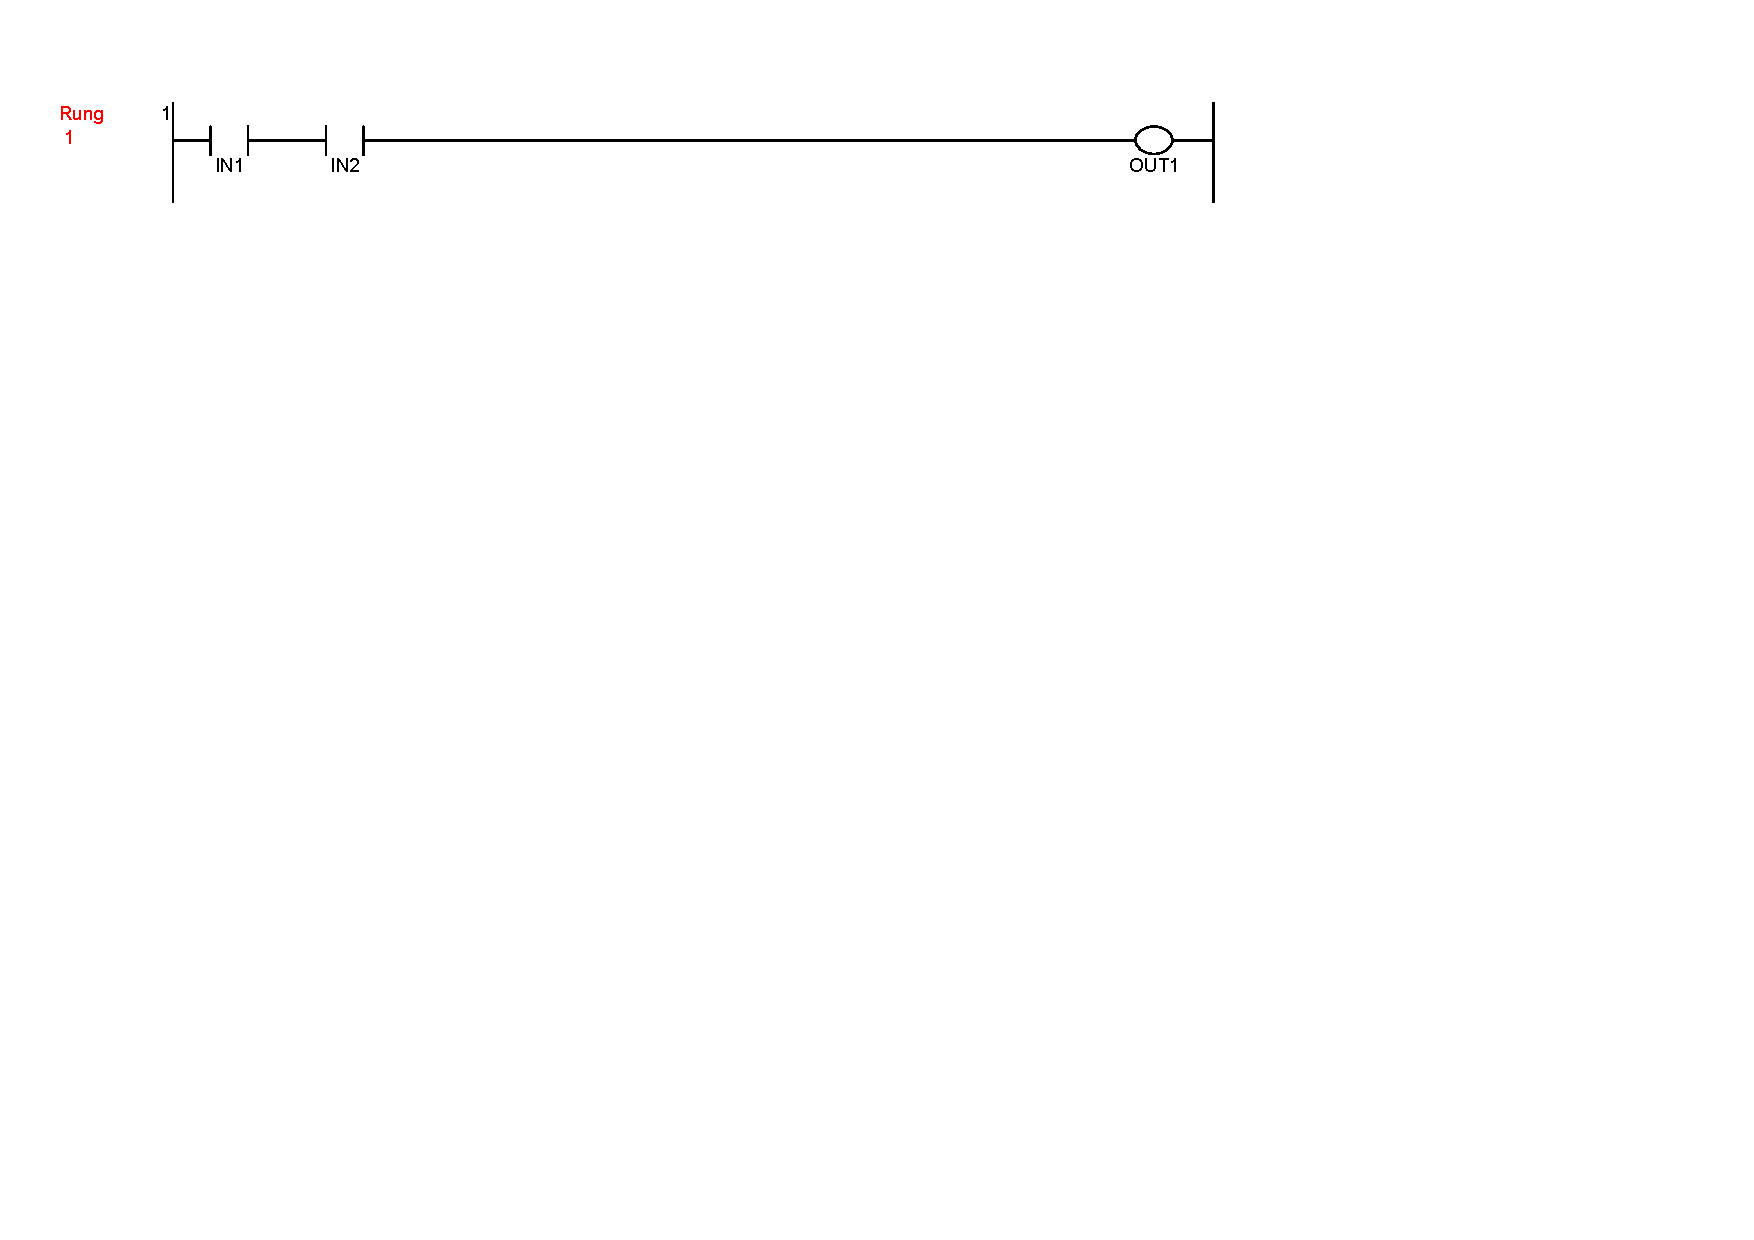
\includegraphics[trim={19pt 489pt 250pt 39pt}, clip, width=0.85\textwidth]{sources/diagramas/WINDLDR_tp3_ej1.pdf}
    \caption{Diagrama Ladder para operación lógica AND (Ejercicio 1).}
    \label{fig.ej1:and}
\end{figure}

\section{Ejercicio 2: Compuerta Lógica O (OR)}
\textbf{Consigna:} Construya un diagrama de contactos que realice la operación lógica O (OR) entre dos entradas y
active una salida.

\textbf{Análisis y Solución:}
Para la función OR, las entradas $I0$ e $I1$ se disponen en ramas paralelas. De este modo, la activación de cualquiera
de las dos entradas (o ambas) energizará la salida $Q0$. El esquema correspondiente se muestra en la figura
\ref{fig.ej2:or}.

\begin{figure}[!ht]
    \centering
    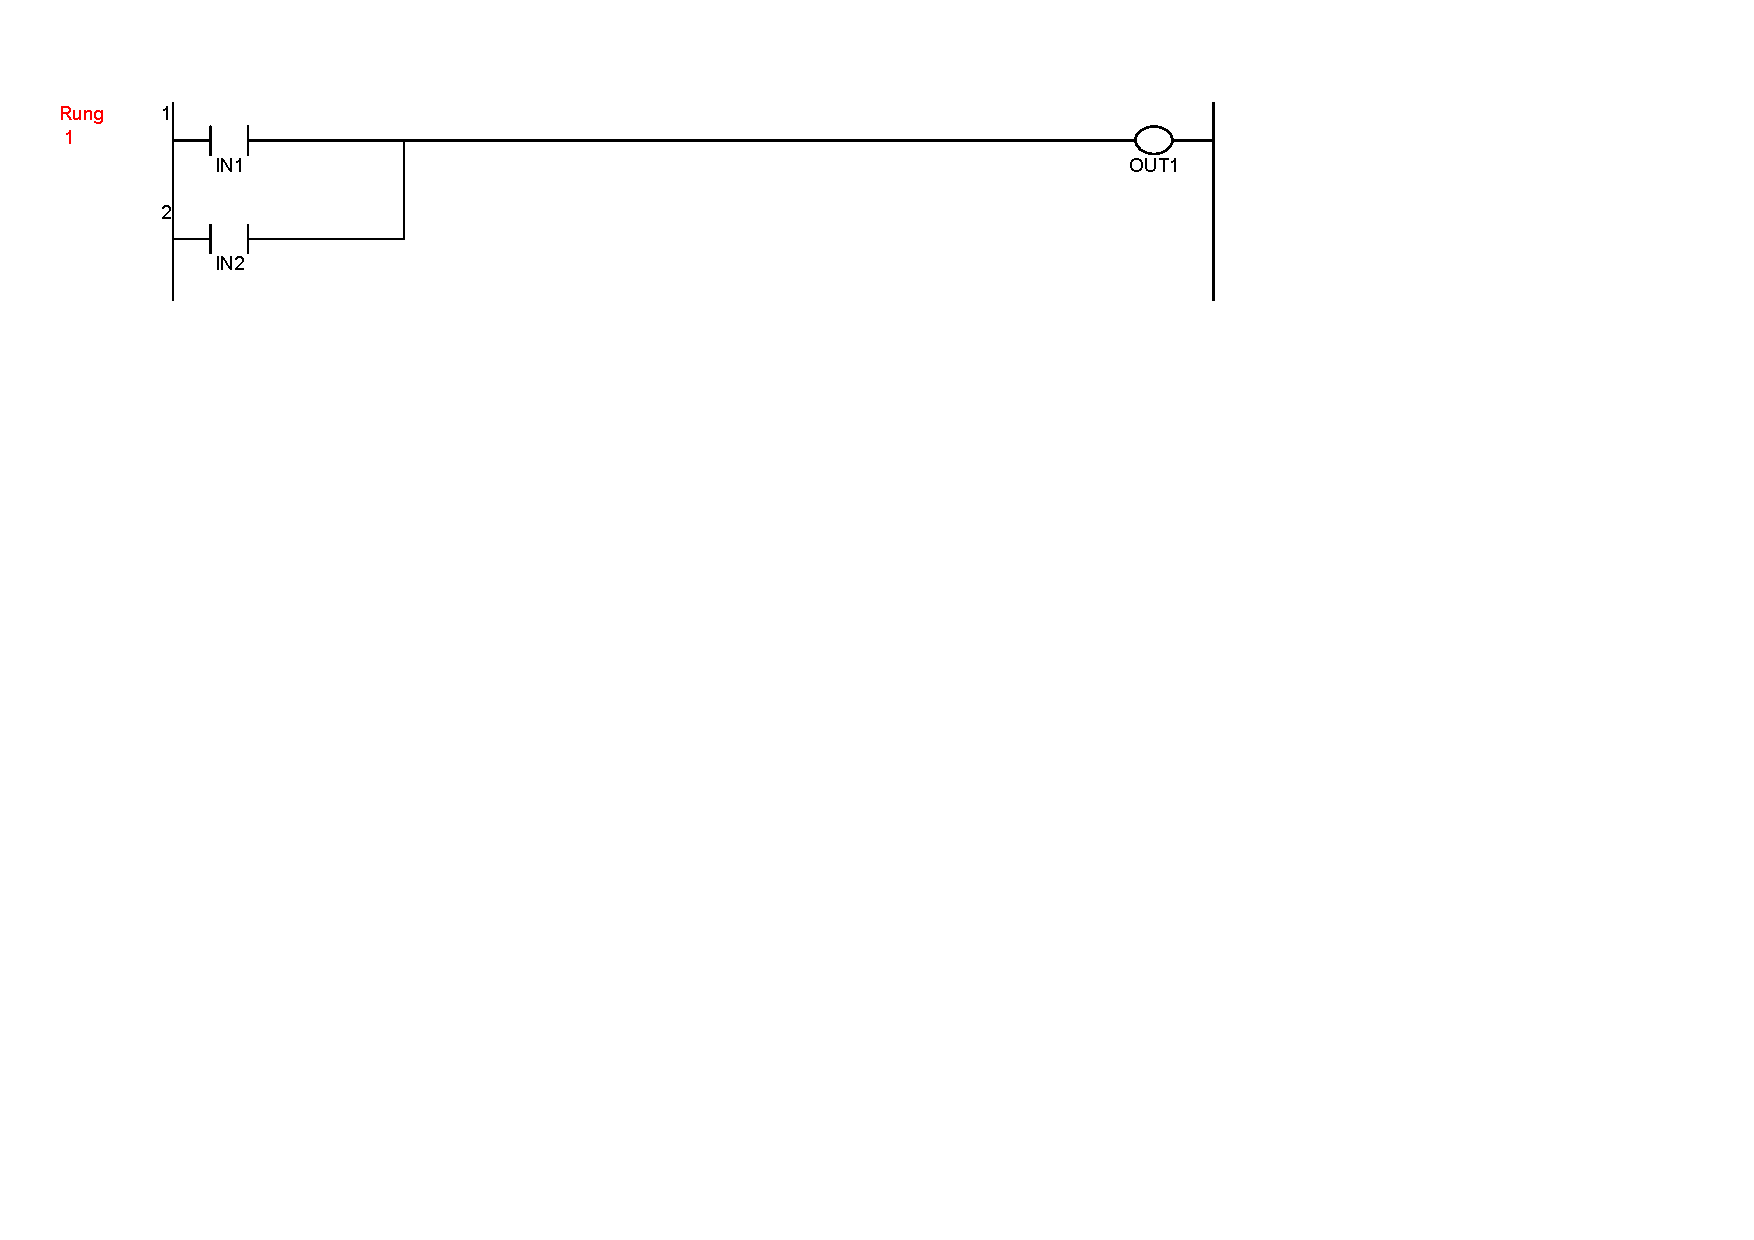
\includegraphics[trim={19pt 441pt 250pt 39pt}, clip, width=0.85\textwidth]{sources/diagramas/WINDLDR_tp3_ej2.pdf}
    \caption{Diagrama Ladder para operación lógica OR (Ejercicio 2).}
    \label{fig.ej2:or}
\end{figure}

\section{Ejercicio 3: Compuerta Lógica NO (NOT)}
\textbf{Consigna:} Construya dos diagramas de contactos distintos que realicen la operación lógica NO (NOT) de una
entrada y active una salida.

\textbf{Análisis y Solución:}
El complemento de una entrada se realiza mediante un contacto normalmente cerrado (NC) o mediante el uso de la
instrucción de reset/inversión de memoria. En la figura \ref{fig.ej3:not} se observan las implementaciones equivalentes.

\begin{figure}[!ht]
    \centering
    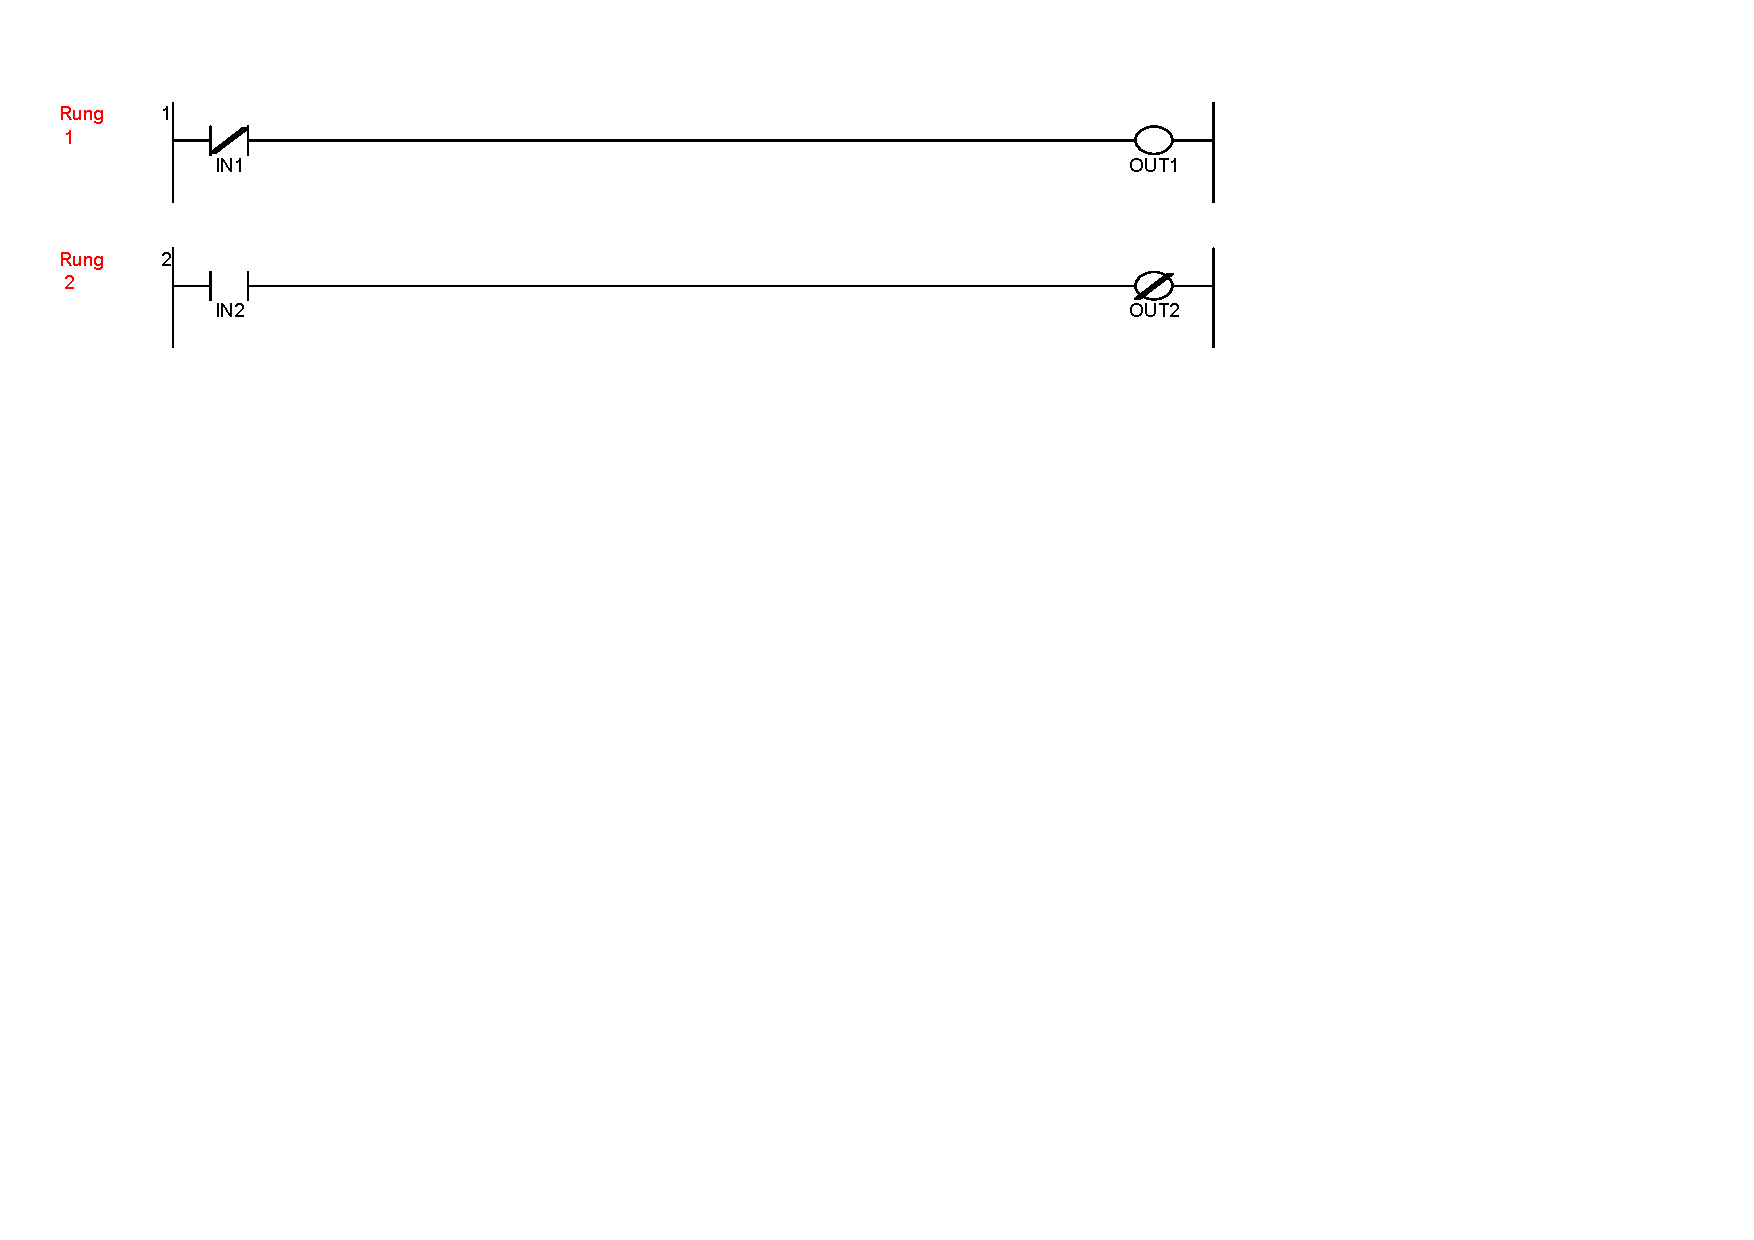
\includegraphics[trim={19pt 418pt 250pt 39pt}, clip, width=0.85\textwidth]{sources/diagramas/WINDLDR_tp3_ej3.pdf}
    \caption{Diagrama Ladder para la función NOT (Ejercicio 3).}
    \label{fig.ej3:not}
\end{figure}

\section{Ejercicio 4: Compuerta Lógica NO Y (NAND)}
\textbf{Consigna:} Construya al menos dos diagramas de contactos distintos que realicen la operación lógica NO Y
(NAND) de dos entradas y active una salida.

\textbf{Análisis y Solución:}
Aplicando las leyes de De Morgan, la expresión $\overline{A \cdot B} = \overline{A} + \overline{B}$. Se puede
implementar colocando dos contactos normalmente cerrados en paralelo, o negando la serie de contactos, tal como se observa
en la figura \ref{fig.ej4:nand}.

\begin{figure}[!ht]
    \centering
    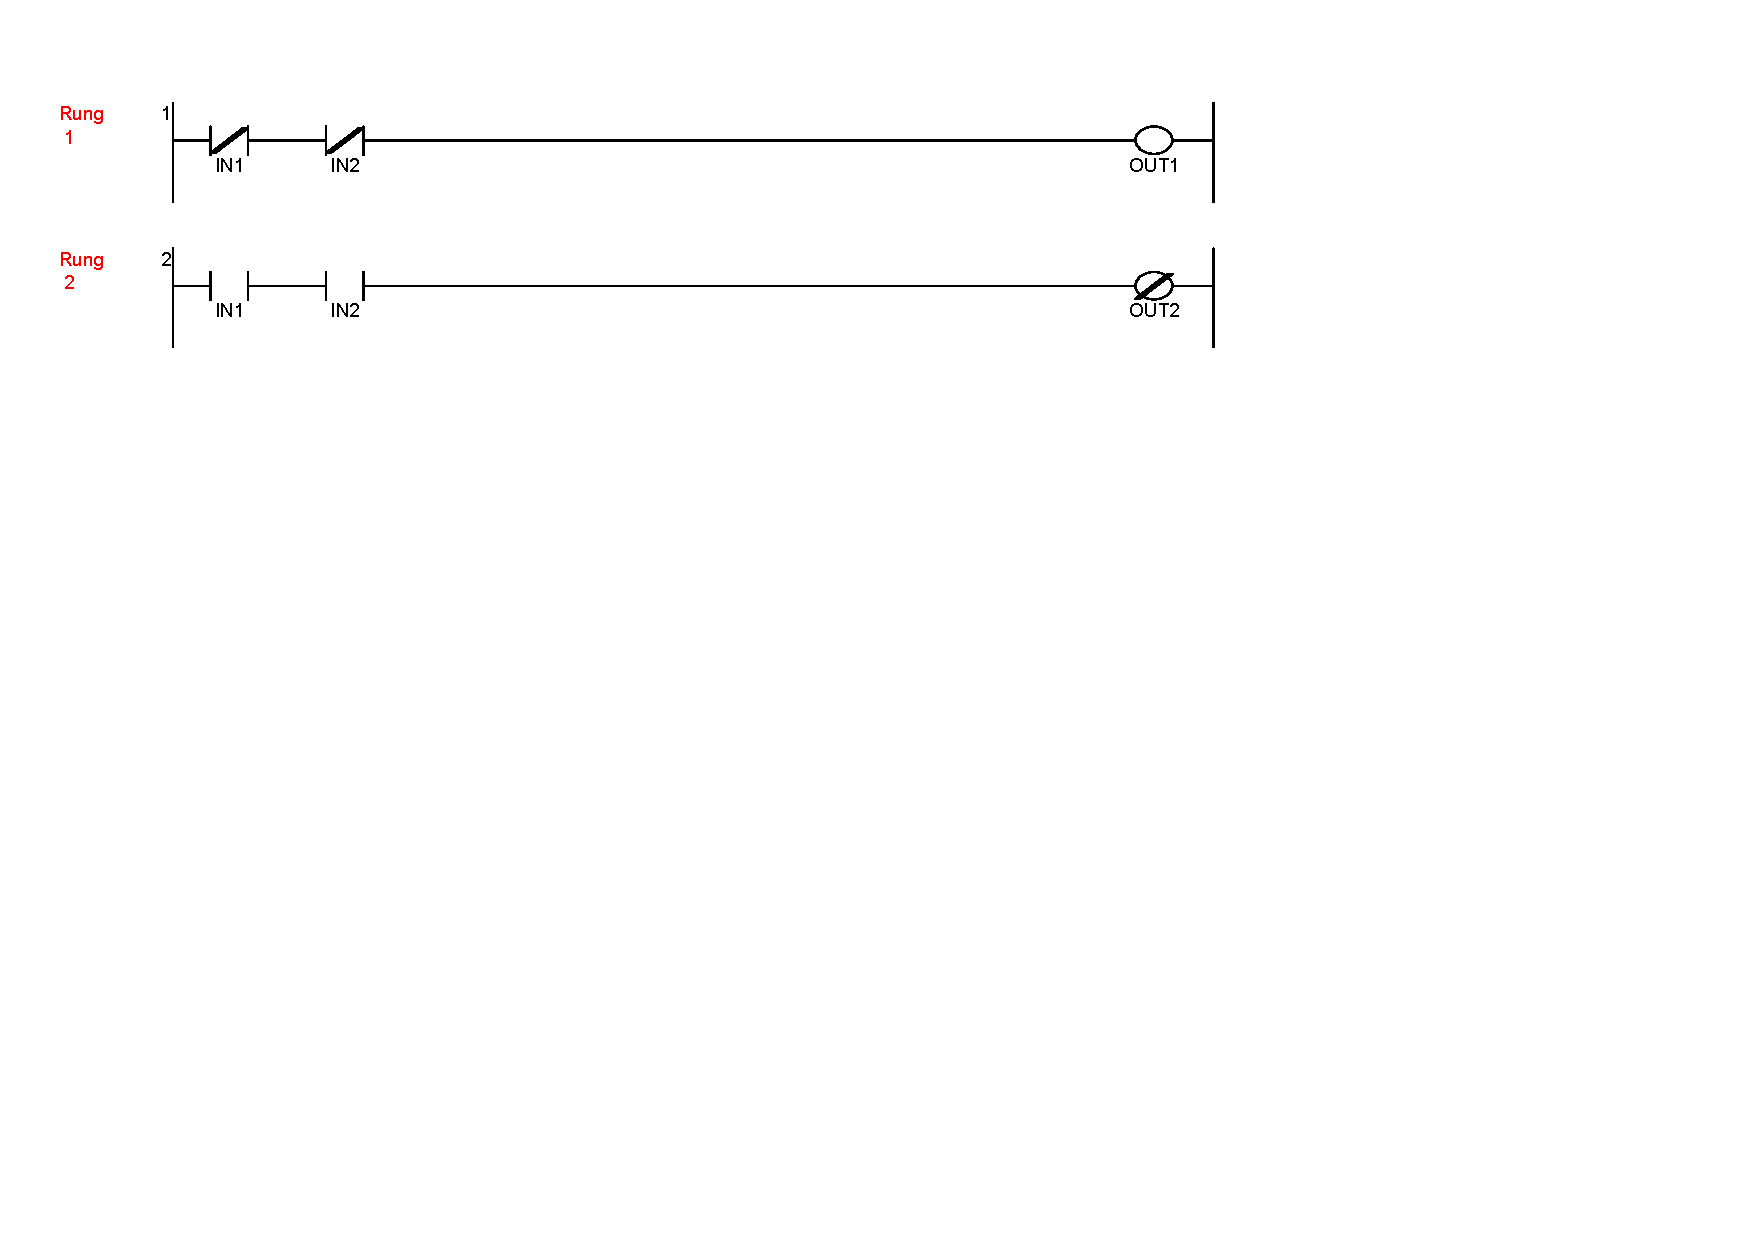
\includegraphics[trim={19pt 418pt 250pt 39pt}, clip, width=0.85\textwidth]{sources/diagramas/WINDLDR_tp3_ej4.pdf}
    \caption{Diagrama Ladder para función NAND (Ejercicio 4).}
    \label{fig.ej4:nand}
\end{figure}

\section{Ejercicio 5: Compuerta Lógica NO O (NOR)}
\textbf{Consigna:} Construya al menos dos diagramas de contactos distintos que realicen la operación lógica NO O
(NOR) de dos entradas y active una salida.

\textbf{Análisis y Solución:}
Por Leyes de De Morgan, $\overline{A + B} = \overline{A} \cdot \overline{B}$. Se implementa conectando dos contactos
normalmente cerrados en serie, tal como se aprecia en el circuito de la figura \ref{fig.ej5:nor}.

\begin{figure}[!ht]
    \centering
    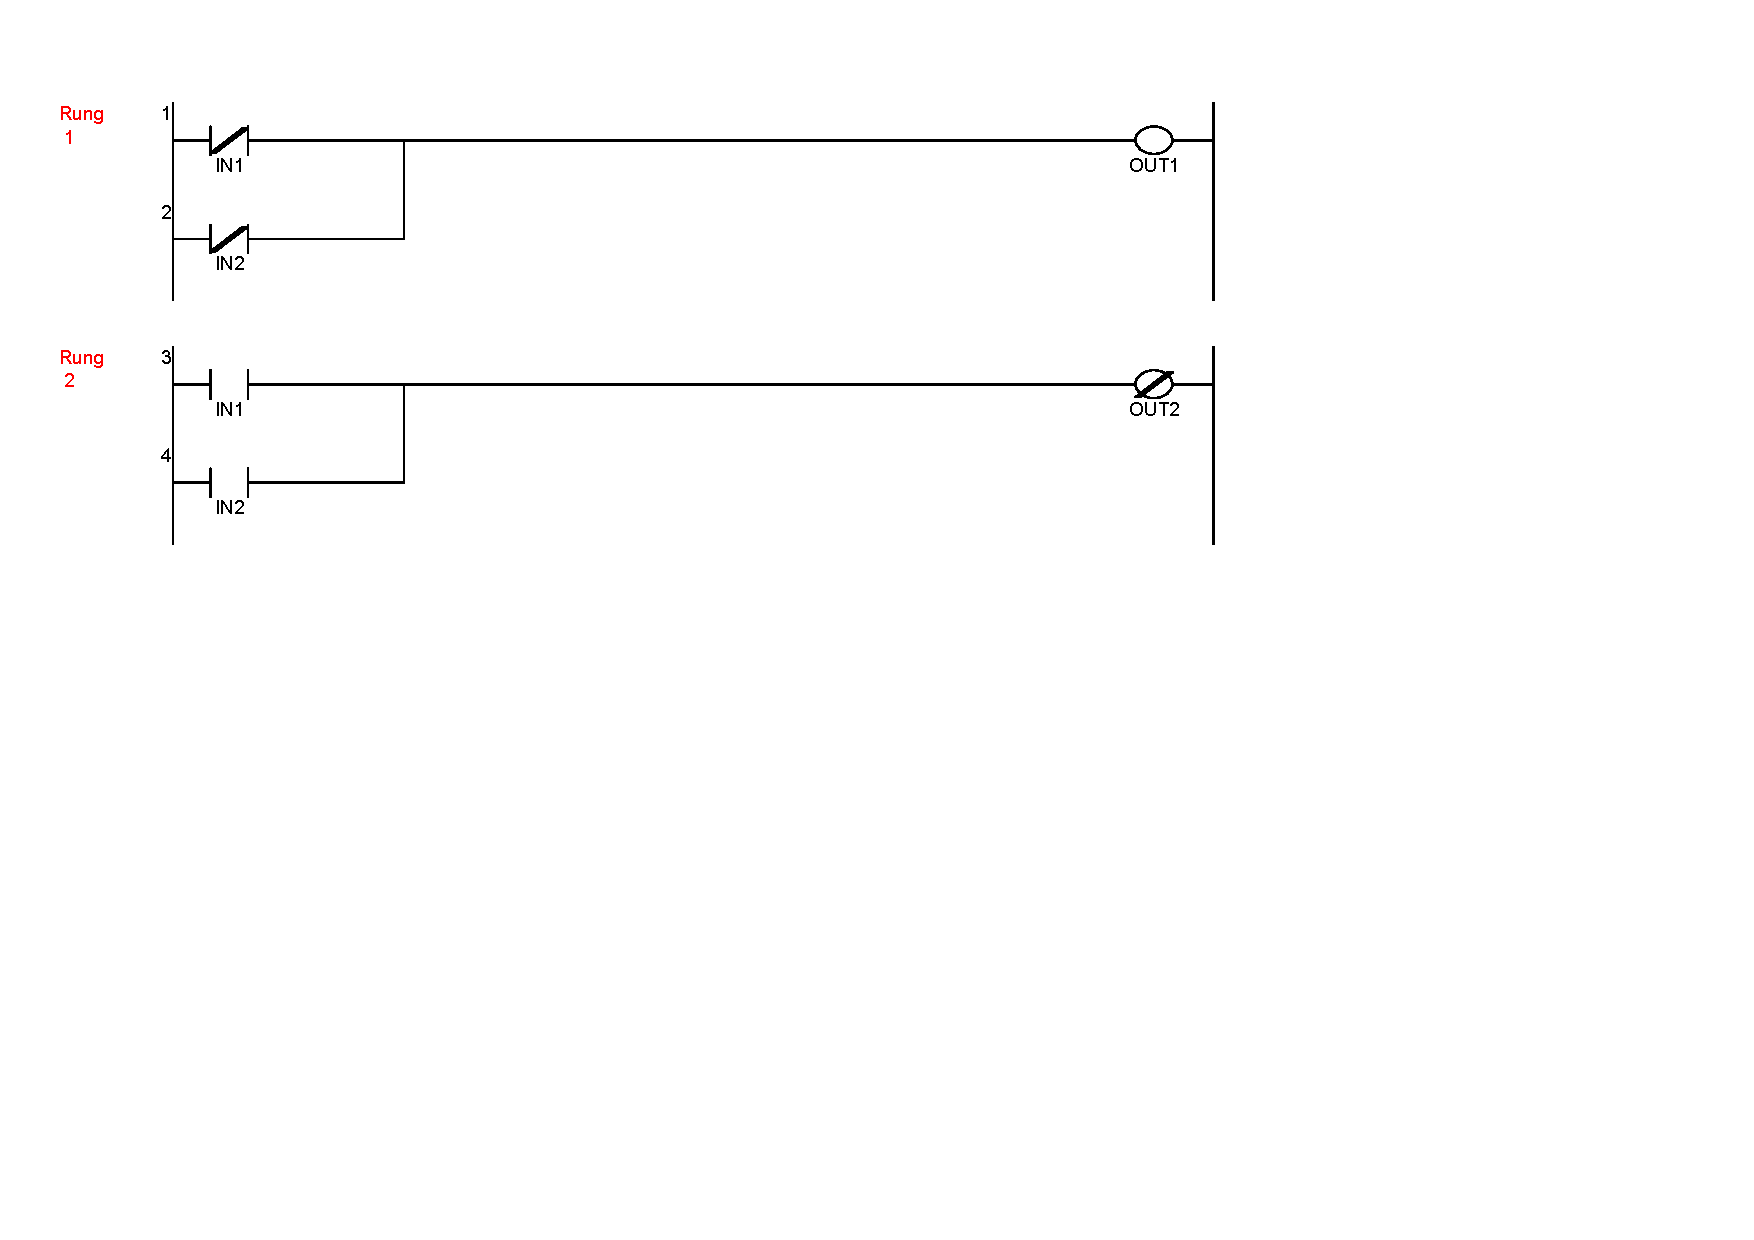
\includegraphics[trim={19pt 324pt 250pt 39pt}, clip, width=0.85\textwidth]{sources/diagramas/WINDLDR_tp3_ej5.pdf}
    \caption{Diagrama Ladder para función NOR (Ejercicio 5).}
    \label{fig.ej5:nor}
\end{figure}

\section{Ejercicio 6: Compuerta O Exclusiva (XOR)}
\textbf{Consigna:} Construya al menos dos diagramas de contactos distintos que realicen la operación lógica O
exclusiva (XOR) de dos entradas y active una salida.

\textbf{Análisis y Solución:}
La ecuación booleana es $Q0 = A \cdot \overline{B} + \overline{A} \cdot B$. Se constituye una red con dos ramas en
paralelo conteniendo contactos combinados (NA y NC), cuya implementación en lenguaje de contactos se refleja en la
figura \ref{fig.ej6:xor}.

\begin{figure}[!ht]
    \centering
    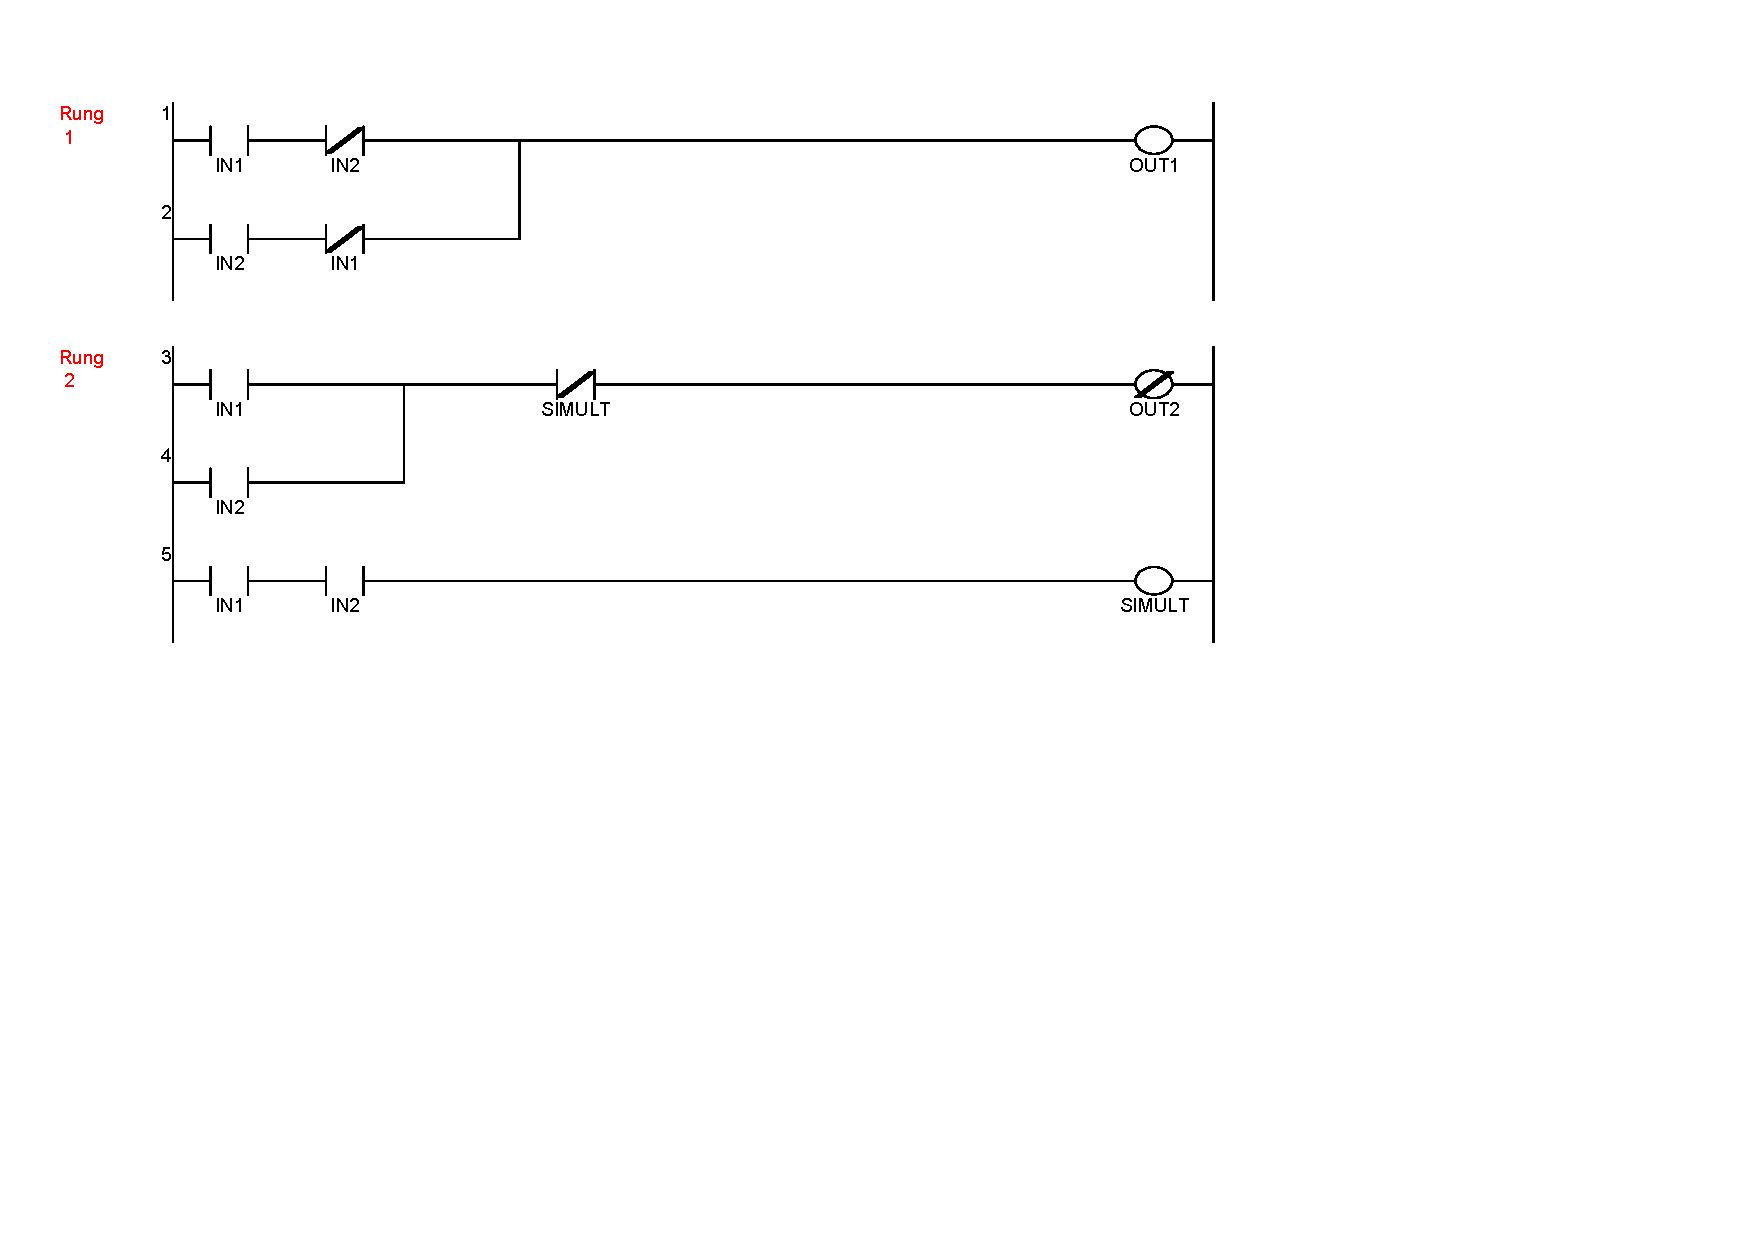
\includegraphics[trim={19pt 277pt 250pt 39pt}, clip, width=0.85\textwidth]{sources/diagramas/WINDLDR_tp3_ej6.pdf}
    \caption{Diagrama Ladder para función XOR (Ejercicio 6).}
    \label{fig.ej6:xor}
\end{figure}

\section{Ejercicio 7: Autoenclavamiento (Start-Stop) vs Flip-Flop SR}
\textbf{Consigna:} Demuestre que el circuito de auto enclavamiento se comporta como un flip-flop Set-Reset, mediante
circuitos equivalentes y en forma analítica.

\textbf{Demostración Analítica:}
Sea $S$ la entrada de marcha (Set, $I0$), $R$ la entrada de parada (Reset, $I1$, normalmente cerrado de parada o
apertura lógica) y $Q$ el estado actual de la salida.
La ecuación de estado del circuito con retención es:
\begin{equation}
    Q_{n+1} = (S + Q_n) \cdot \overline{R}
    \label{eq.ej7:retencion}
\end{equation}
La tabla de verdad correspondiente para dicha ecuación lógica se detalla en la tabla \ref{tab.ej7:tabla}:
\begin{table}[!ht]
    \centering
    \begin{tabular}{|c|c|c|c|}
        \hline
        $S$ ($I0$) & $R$ ($I1$) & $Q_n$ & $Q_{n+1}$ \\ \hline
        0 & 0 & 0 & 0 \\
        0 & 0 & 1 & 1 (Memoria) \\
        1 & 0 & X & 1 (Set) \\
        X & 1 & X & 0 (Reset prioritario) \\ \hline
    \end{tabular}
    \caption{Tabla de verdad de retención autoenclavada.}
    \label{tab.ej7:tabla}
\end{table}

Esta relación matemática responde exactamente a la tabla característica de un Flip-Flop SR con prioridad al reset.

\section{Ejercicio 8: Flip-Flop Toggle (Biestable T)}
\textbf{Consigna:} Construya un diagrama de contactos que realice la operación de un flip-flop Toggle.

\textbf{Análisis y Solución:}
El flip-flop Toggle conmuta el estado de la salida $Q0$ en cada flanco ascendente de la entrada de pulso $I0$,
apoyándose en marcas auxiliares o detección de flancos SOTU, según se ilustra en el diagrama de la figura
\ref{fig.ej8:toggle}.

\begin{figure}[!ht]
    \centering
    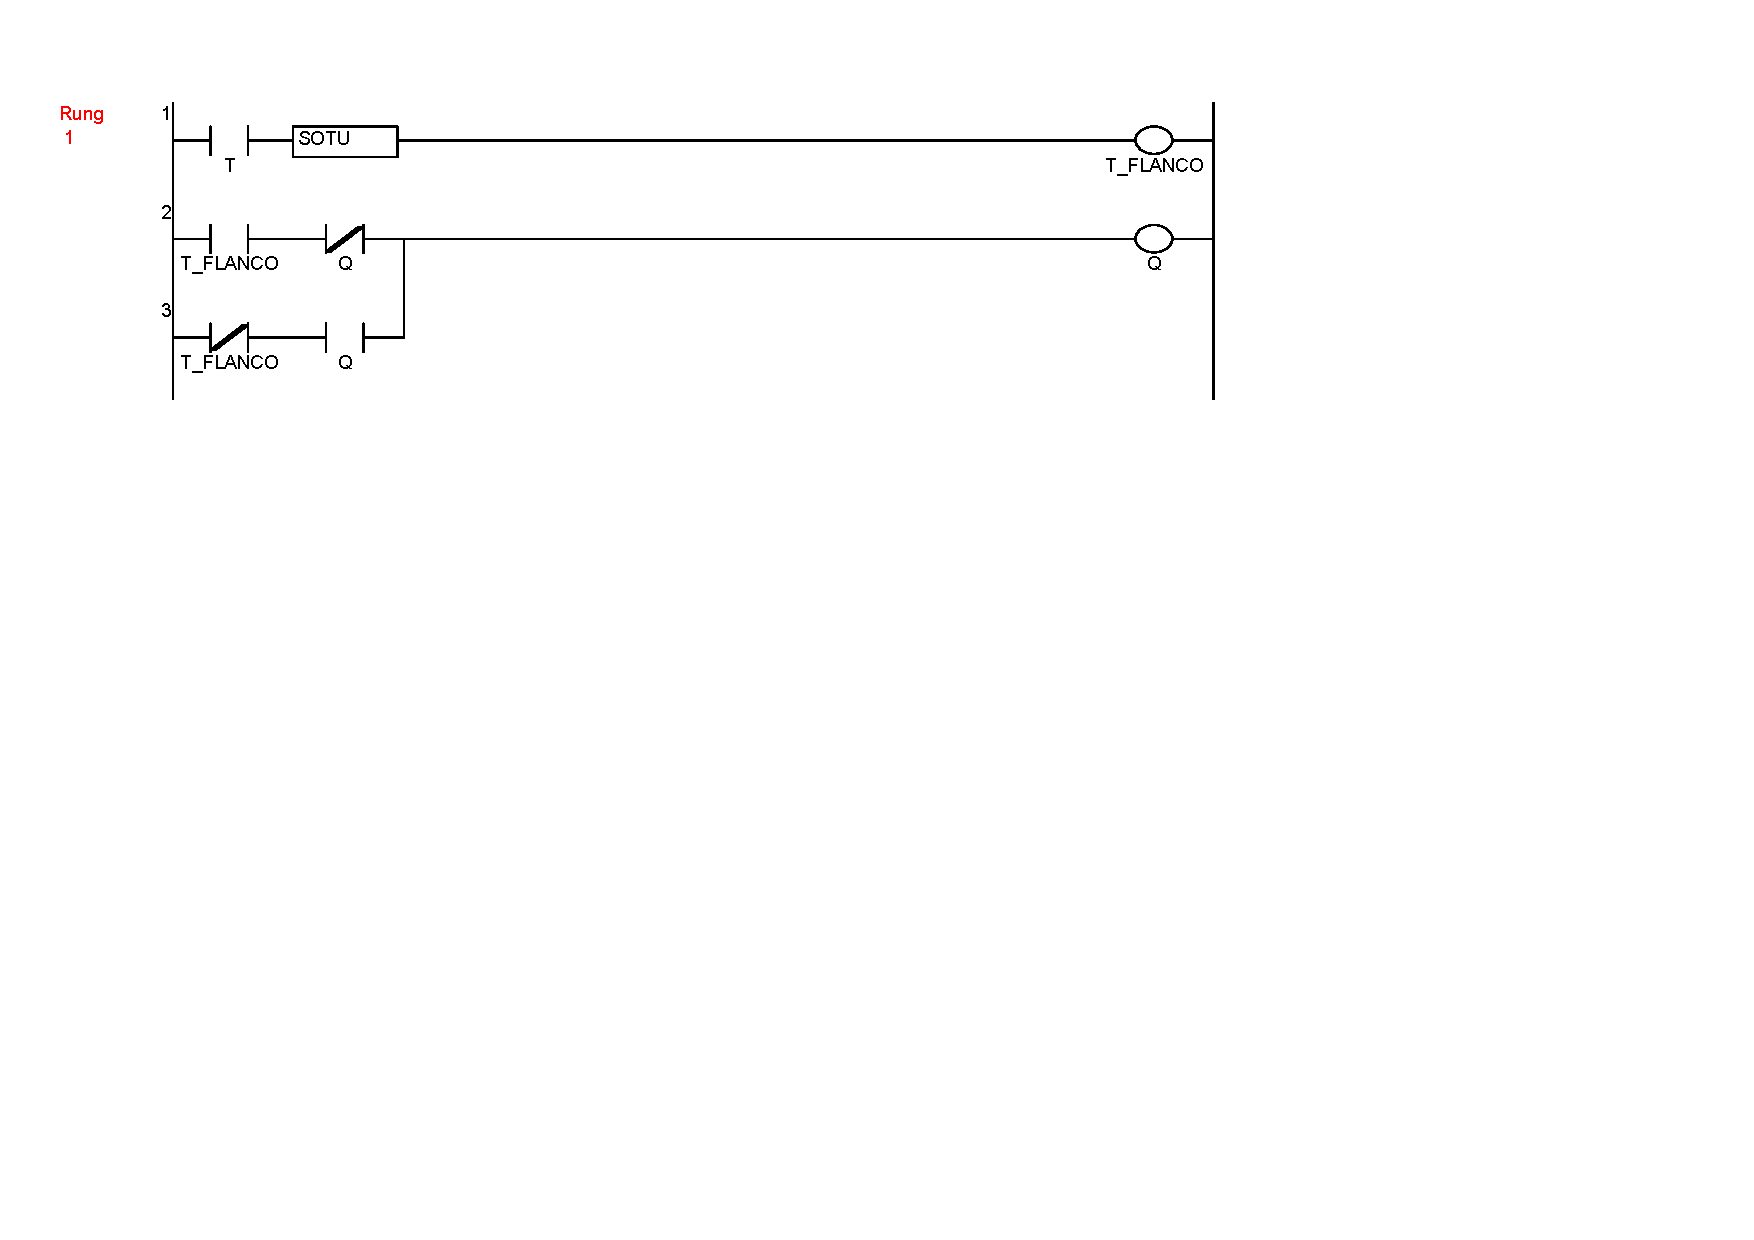
\includegraphics[trim={19pt 394pt 250pt 39pt}, clip, width=0.85\textwidth]{sources/diagramas/WINDLDR_tp3_ej8.pdf}
    \caption{Diagrama Ladder para Flip-Flop Toggle (Ejercicio 8).}
    \label{fig.ej8:toggle}
\end{figure}

\section{Ejercicio 9: Control de Nivel de un Tanque de Agua}
\textbf{Consigna:} Cuando se activa el sensor $I0$ (nivel bajo), se enciende la bomba $Q0$ hasta que se cierre el sensor
$I1$ (nivel alto). En la bomba se cuenta con un sensor de presencia de líquido ($I2$) que debe permitir funcionar a la
bomba solo si hay agua en la tubería.

\textbf{Análisis y Solución:}
Se implementa un ciclo de histéresis mediante retención donde la marcha la dicta $I0$ y la parada $I1$. El sensor $I2$ se
ubica en serie con la salida $Q0$, garantizando el apagado automático inmediato si falla el suministro. El diagrama
Ladder correspondiente se muestra en la figura \ref{fig.ej9:tanque}.

\begin{figure}[!ht]
    \centering
    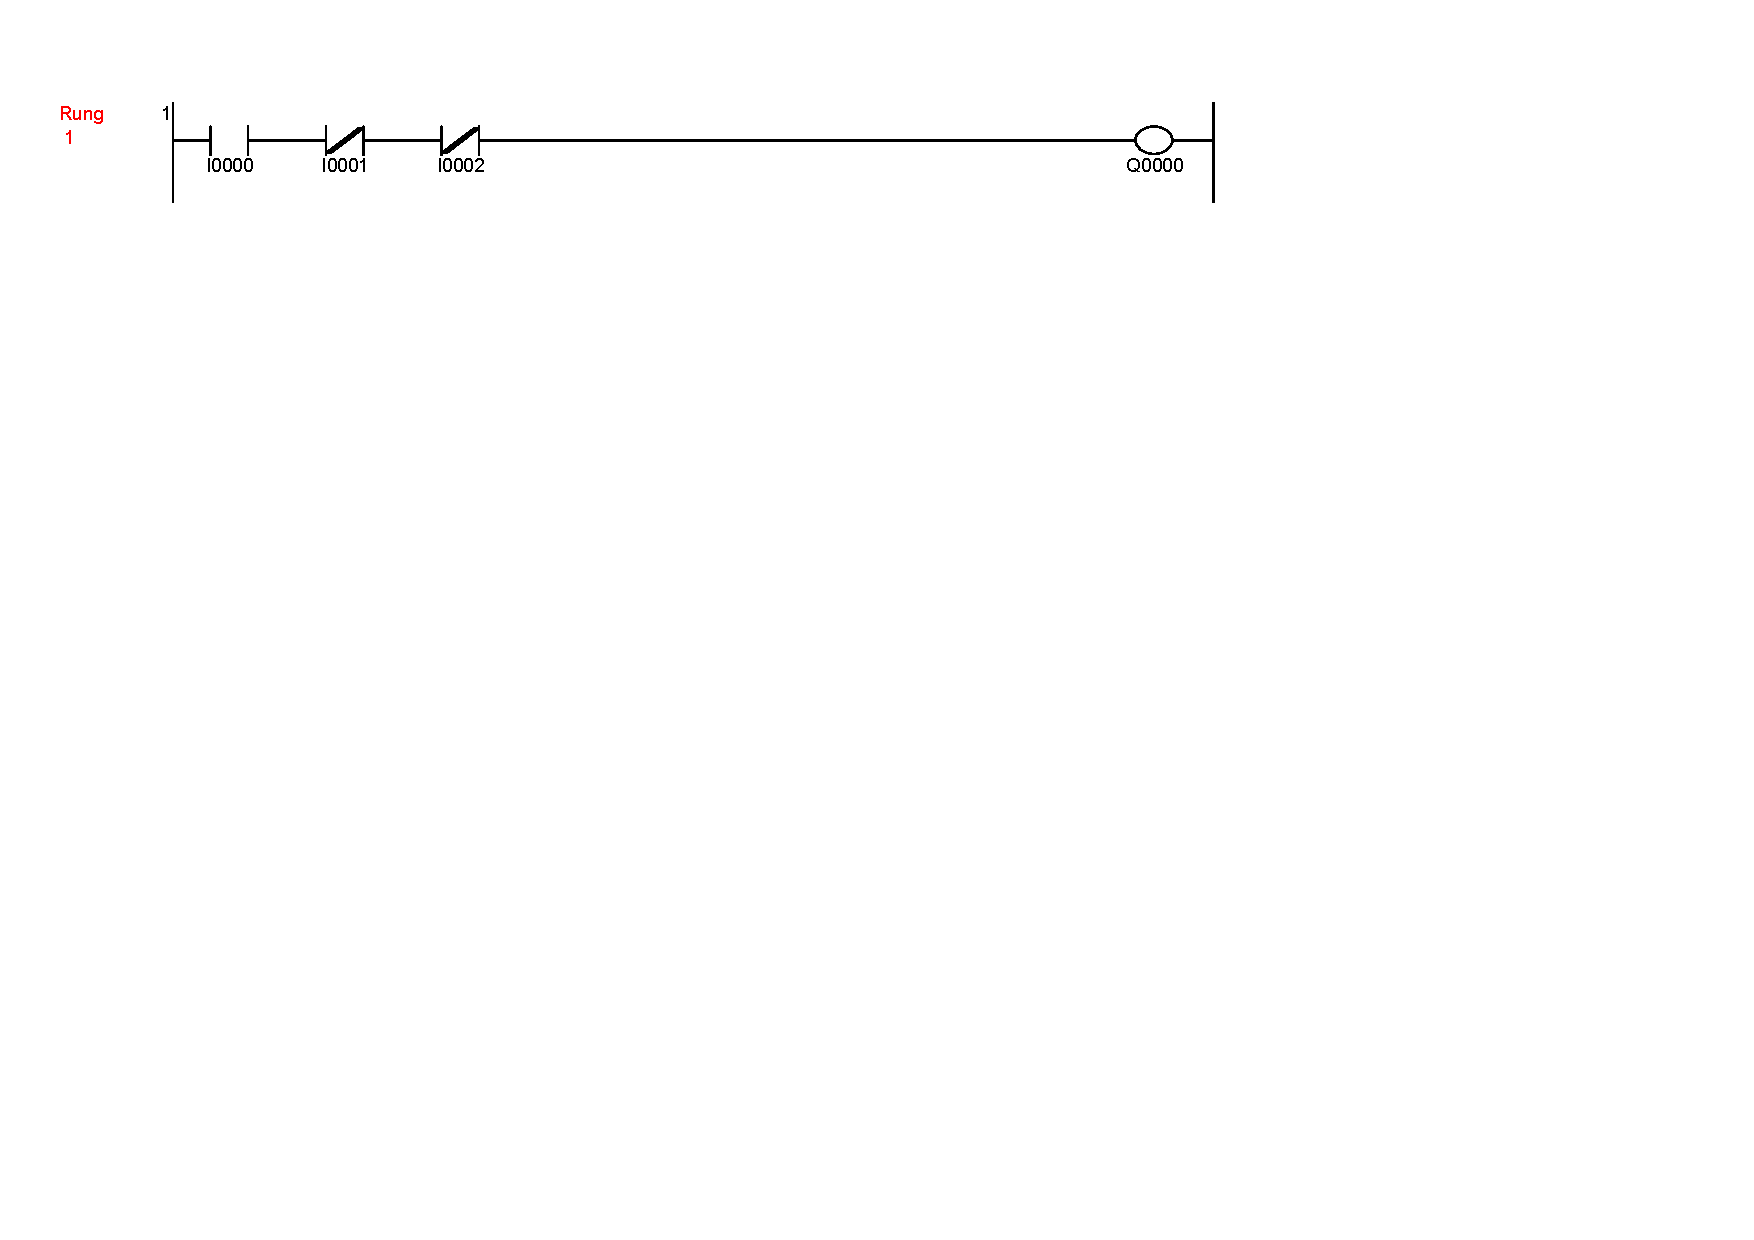
\includegraphics[trim={19pt 489pt 250pt 39pt}, clip, width=0.85\textwidth]{sources/diagramas/WINDLDR_tp3_ej9.pdf}
    \caption{Diagrama Ladder para el control de bomba de agua (Ejercicio 9).}
    \label{fig.ej9:tanque}
\end{figure}

\section{Ejercicio 10: Montacargas de Dos Posiciones}
\textbf{Consigna:} Sensores de posición $Sa$ ($I2$) y $Sb$ ($I3$) indican la posición. Los pulsadores $Pa$ ($I0$) y
$Pb$ ($I1$) activarán el motor para subir/bajar a través de las salidas $Q0$ y $Q1$.

\textbf{Análisis y Solución:}
Se establecen enclavamientos cruzados eléctricos y lógicos entre las salidas $Q0$ (subir) y $Q1$ (bajar) para evitar
cortocircuitos o comandos simultáneos, deteniendo el movimiento automáticamente mediante los finales de carrera. La
solución en lenguaje Ladder se aprecia en la figura \ref{fig.ej10:montacargas}.

\begin{figure}[!ht]
    \centering
    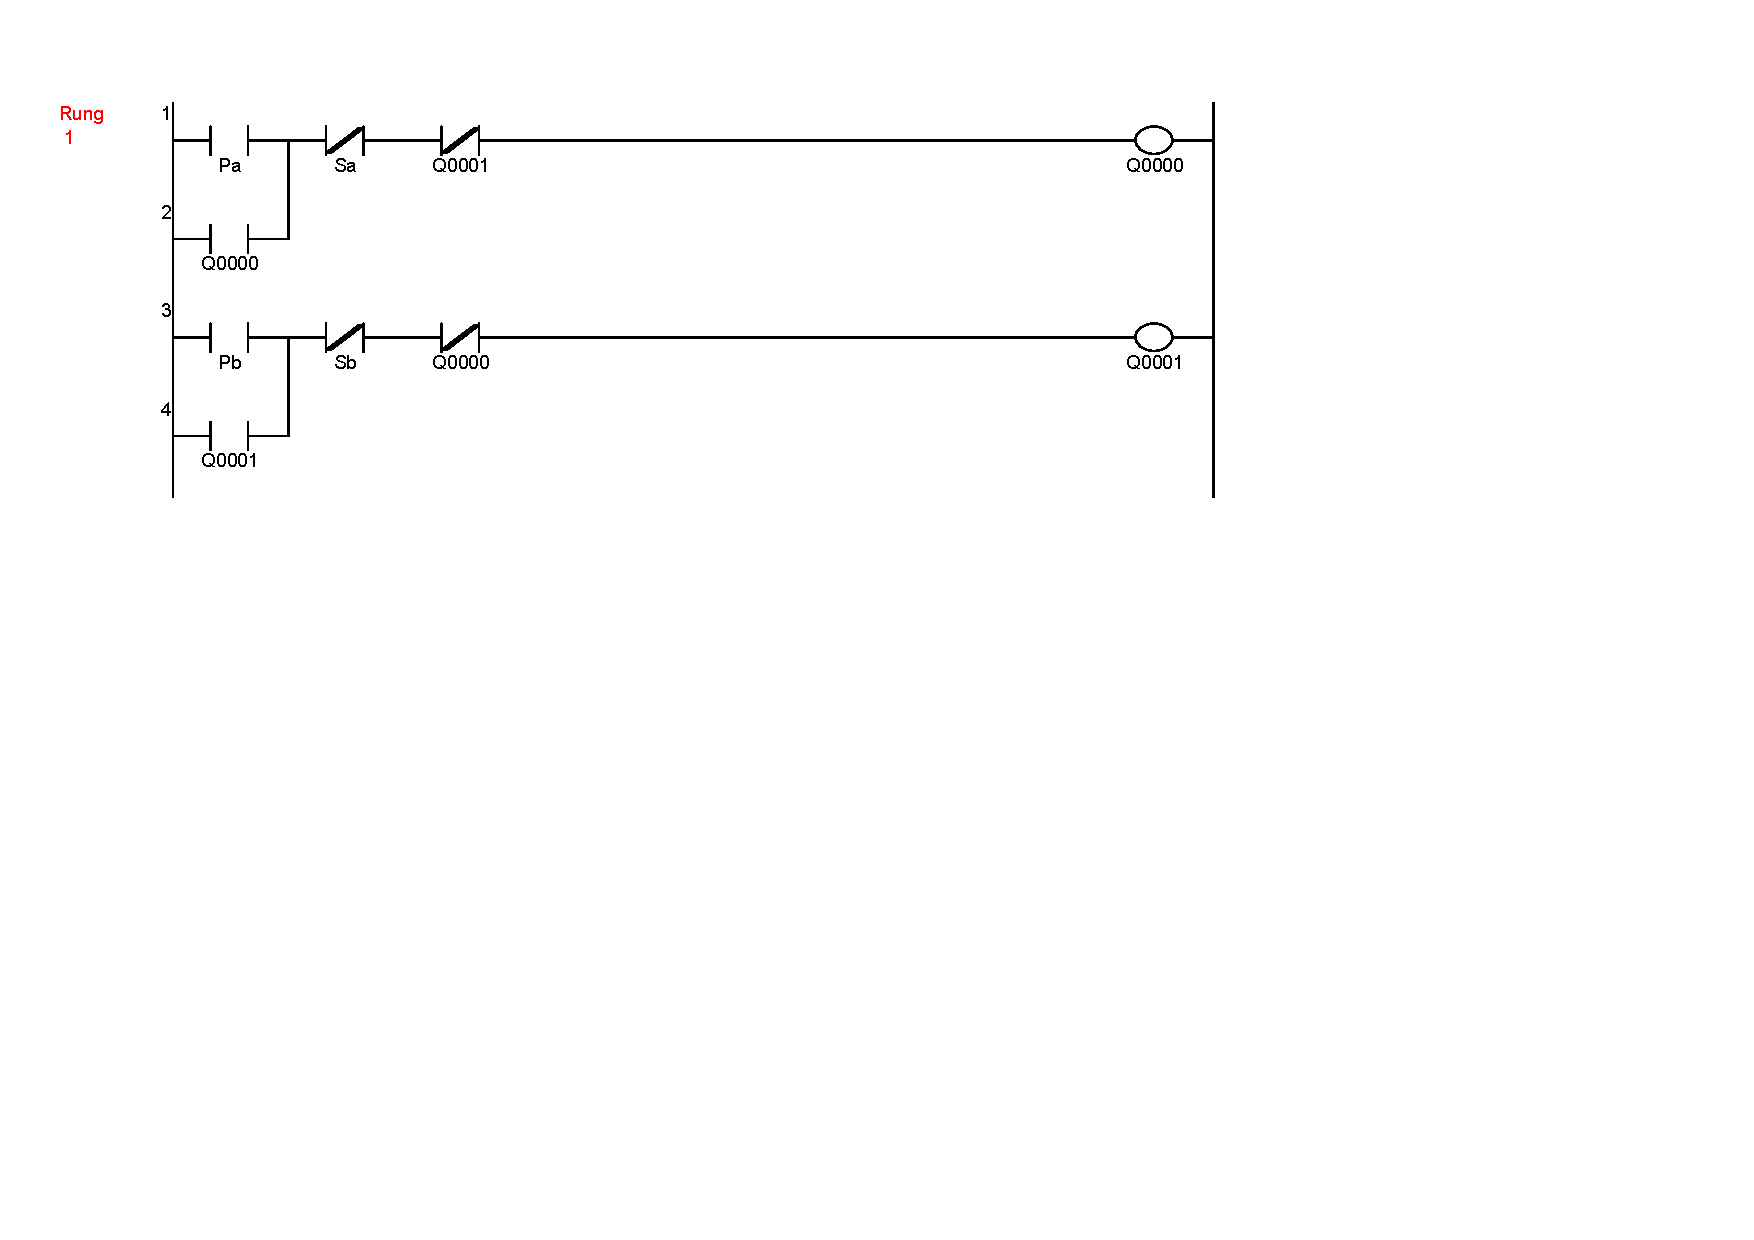
\includegraphics[trim={19pt 347pt 250pt 39pt}, clip, width=0.85\textwidth]{sources/diagramas/WINDLDR_tp3_ej10.pdf}
    \caption{Diagrama Ladder para Montacargas de 2 Posiciones (Ejercicio 10).}
    \label{fig.ej10:montacargas}
\end{figure}

\section{Ejercicio 11: Temporizador Encendido Inmediato y Apagado Retardado (10s)}
\textbf{Consigna:} Diseñe un diagrama ladder que encienda la salida $Q0$ inmediatamente al energizar $I0$ (pulsador
momentáneo) y luego se apague tras $10\,\text{s}$.

\textbf{Análisis y Solución:}
La pulsación de $I0$ encierra un enclavamiento para $Q0$ que a la vez dispara el temporizador $T0$ preseteado en
$100$ ($10\,\text{s}$). Al expirar $T0$, un contacto NC abre la rama de retención de $Q0$. La arquitectura de lógica de
control se presenta en la figura \ref{fig.ej11:temp10s}.

\begin{figure}[!ht]
    \centering
    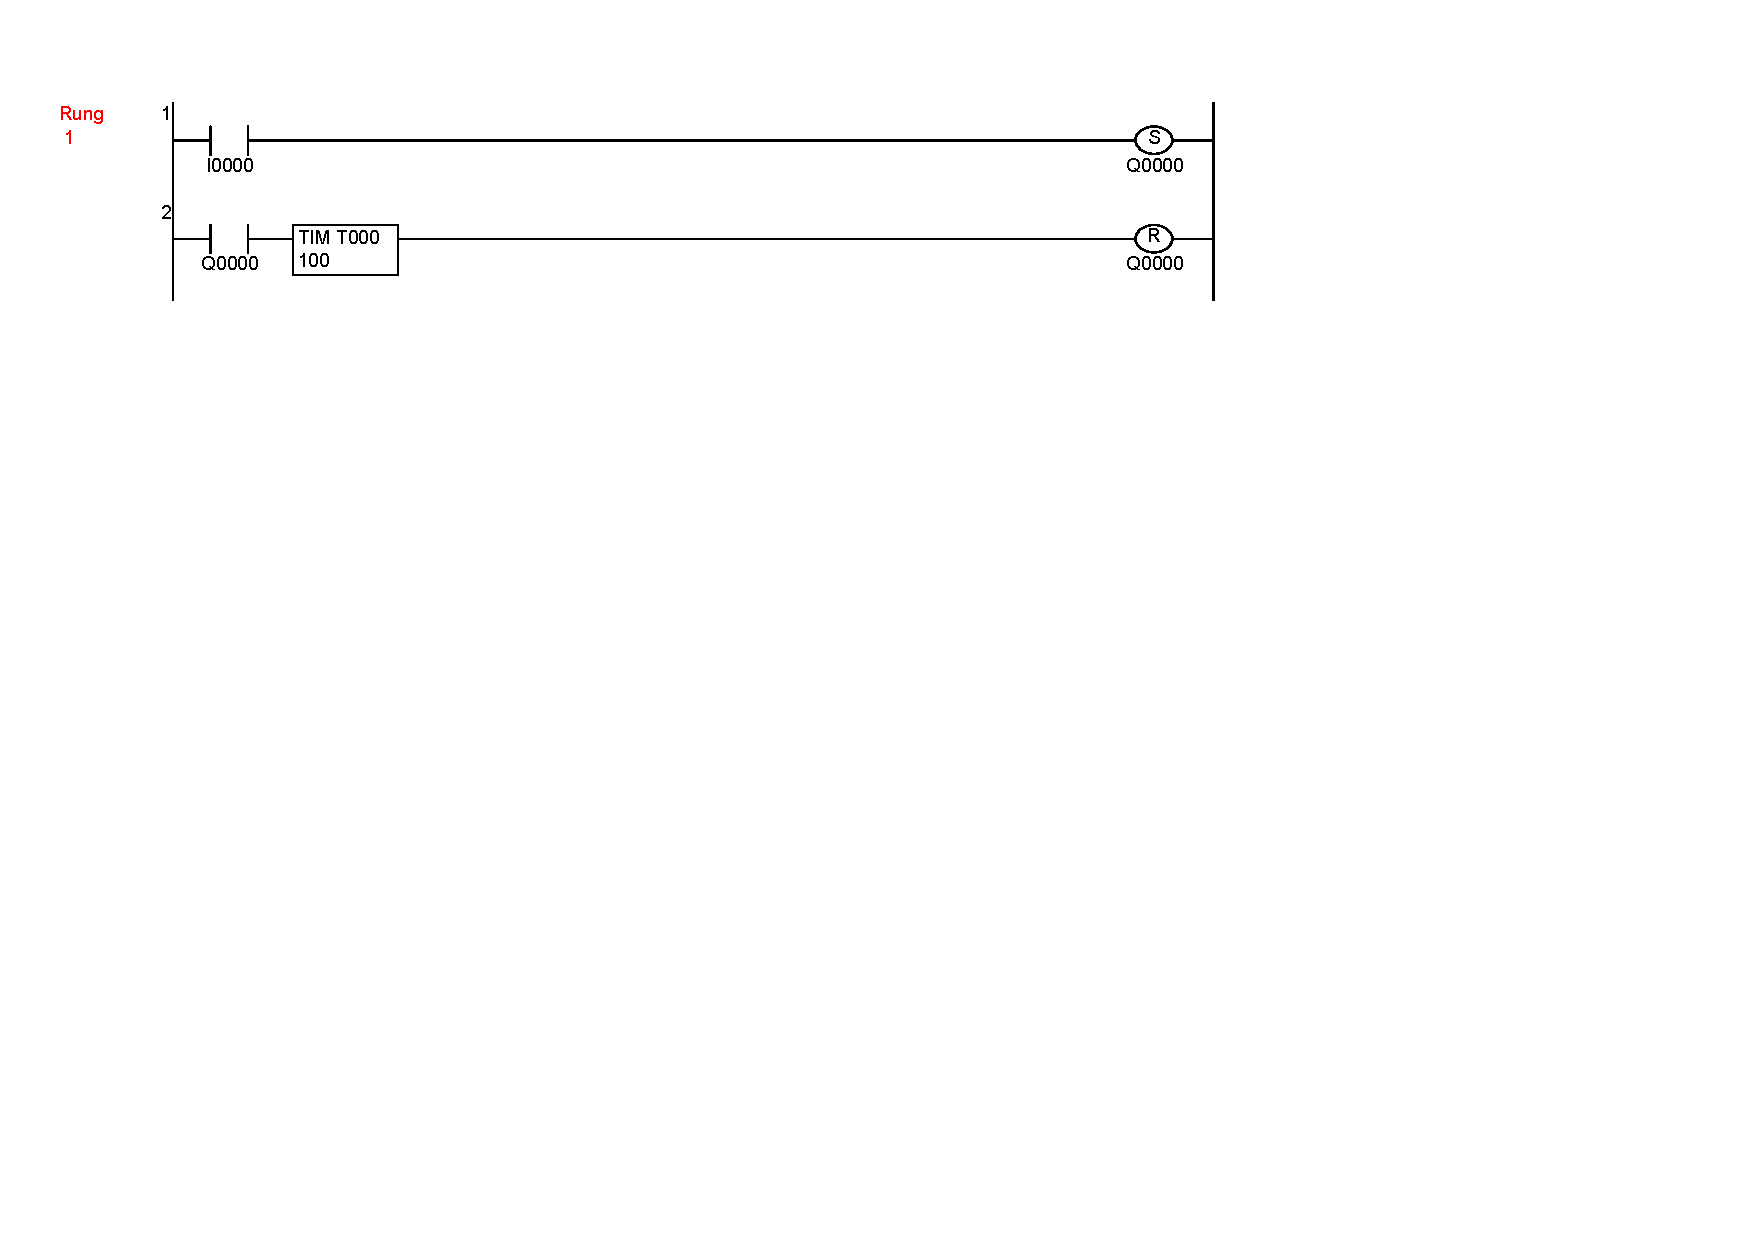
\includegraphics[trim={19pt 441pt 250pt 39pt}, clip, width=0.85\textwidth]{sources/diagramas/WINDLDR_tp3_ej11.pdf}
    \caption{Diagrama Ladder para temporización de $10\,\text{s}$ (Ejercicio 11).}
    \label{fig.ej11:temp10s}
\end{figure}

\section{Ejercicio 12: Encendido Retardado y Apagado Retardado}
\textbf{Consigna:} Encender la salida $Q0$ $10\,\text{s}$ después de energizar $I0$ y luego apagar $5\,\text{s}$
después de que se active $I1$ (entradas momentáneas).

\textbf{Análisis y Solución:}
Se utilizan dos temporizadores ($T0$ de $10\,\text{s}$ para retardo a la conexión y $T1$ de $5\,\text{s}$ para retardo a la
desconexión tras el pulso $I1$). La interconexión lógica completa se muestra en la figura \ref{fig.ej12:tempdoble}.

\begin{figure}[!ht]
    \centering
    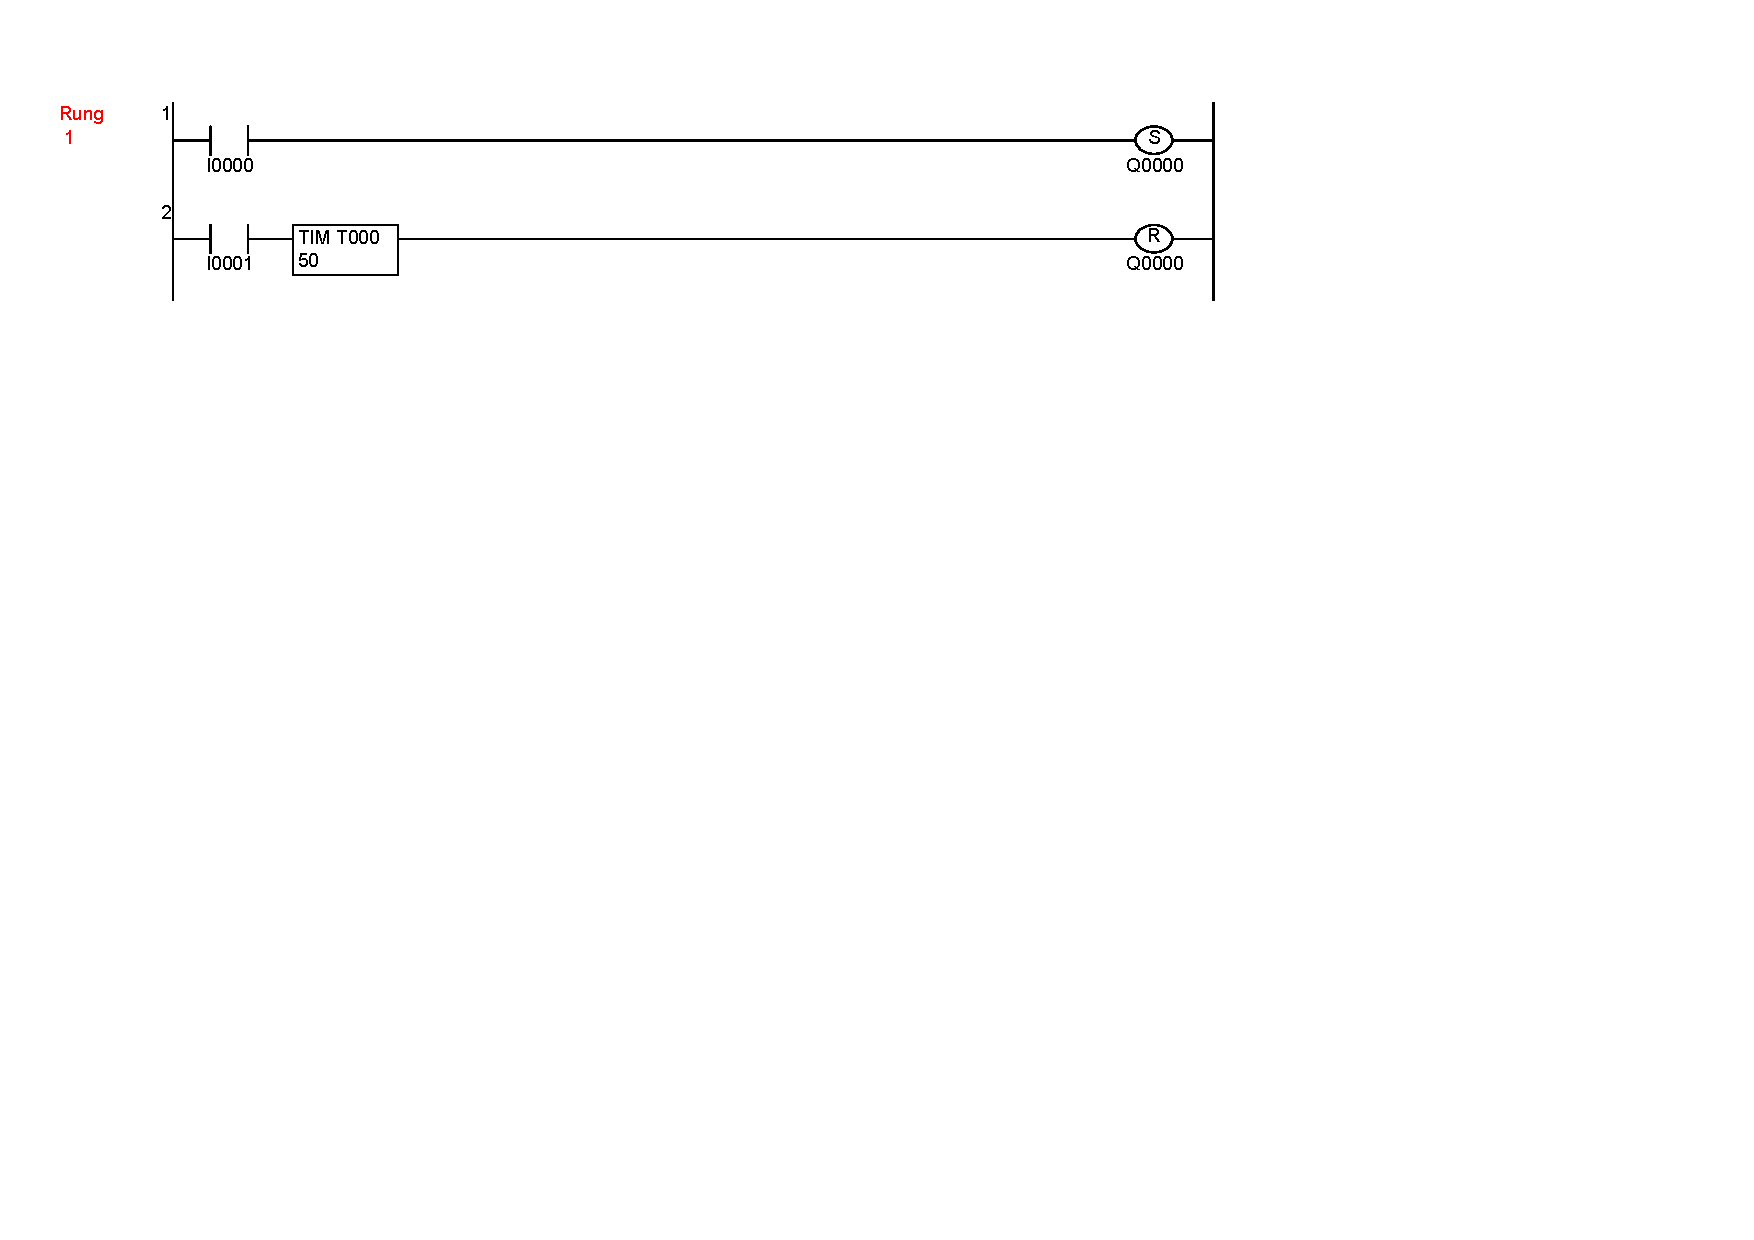
\includegraphics[trim={19pt 441pt 250pt 39pt}, clip, width=0.85\textwidth]{sources/diagramas/WINDLDR_tp3_ej12.pdf}
    \caption{Diagrama Ladder para secuencia de temporización doble (Ejercicio 12).}
    \label{fig.ej12:tempdoble}
\end{figure}

\section{Ejercicio 13: Generador de Pulsos Cíclicos (Oscilador 4s)}
\textbf{Consigna:} Diseñe un temporizador que automáticamente genere un pulso cada $4\,\text{s}$ activado por $I0$.

\textbf{Análisis y Solución:}
Se recurre a una configuración autorestablible con un temporizador $T0$ configurado a $40$ ($4\,\text{s}$), donde el
contacto normalmente cerrado del propio $T0$ realimenta su habilitación, tal como se observa en la figura
\ref{fig.ej13:oscilador}.

\begin{figure}[!ht]
    \centering
    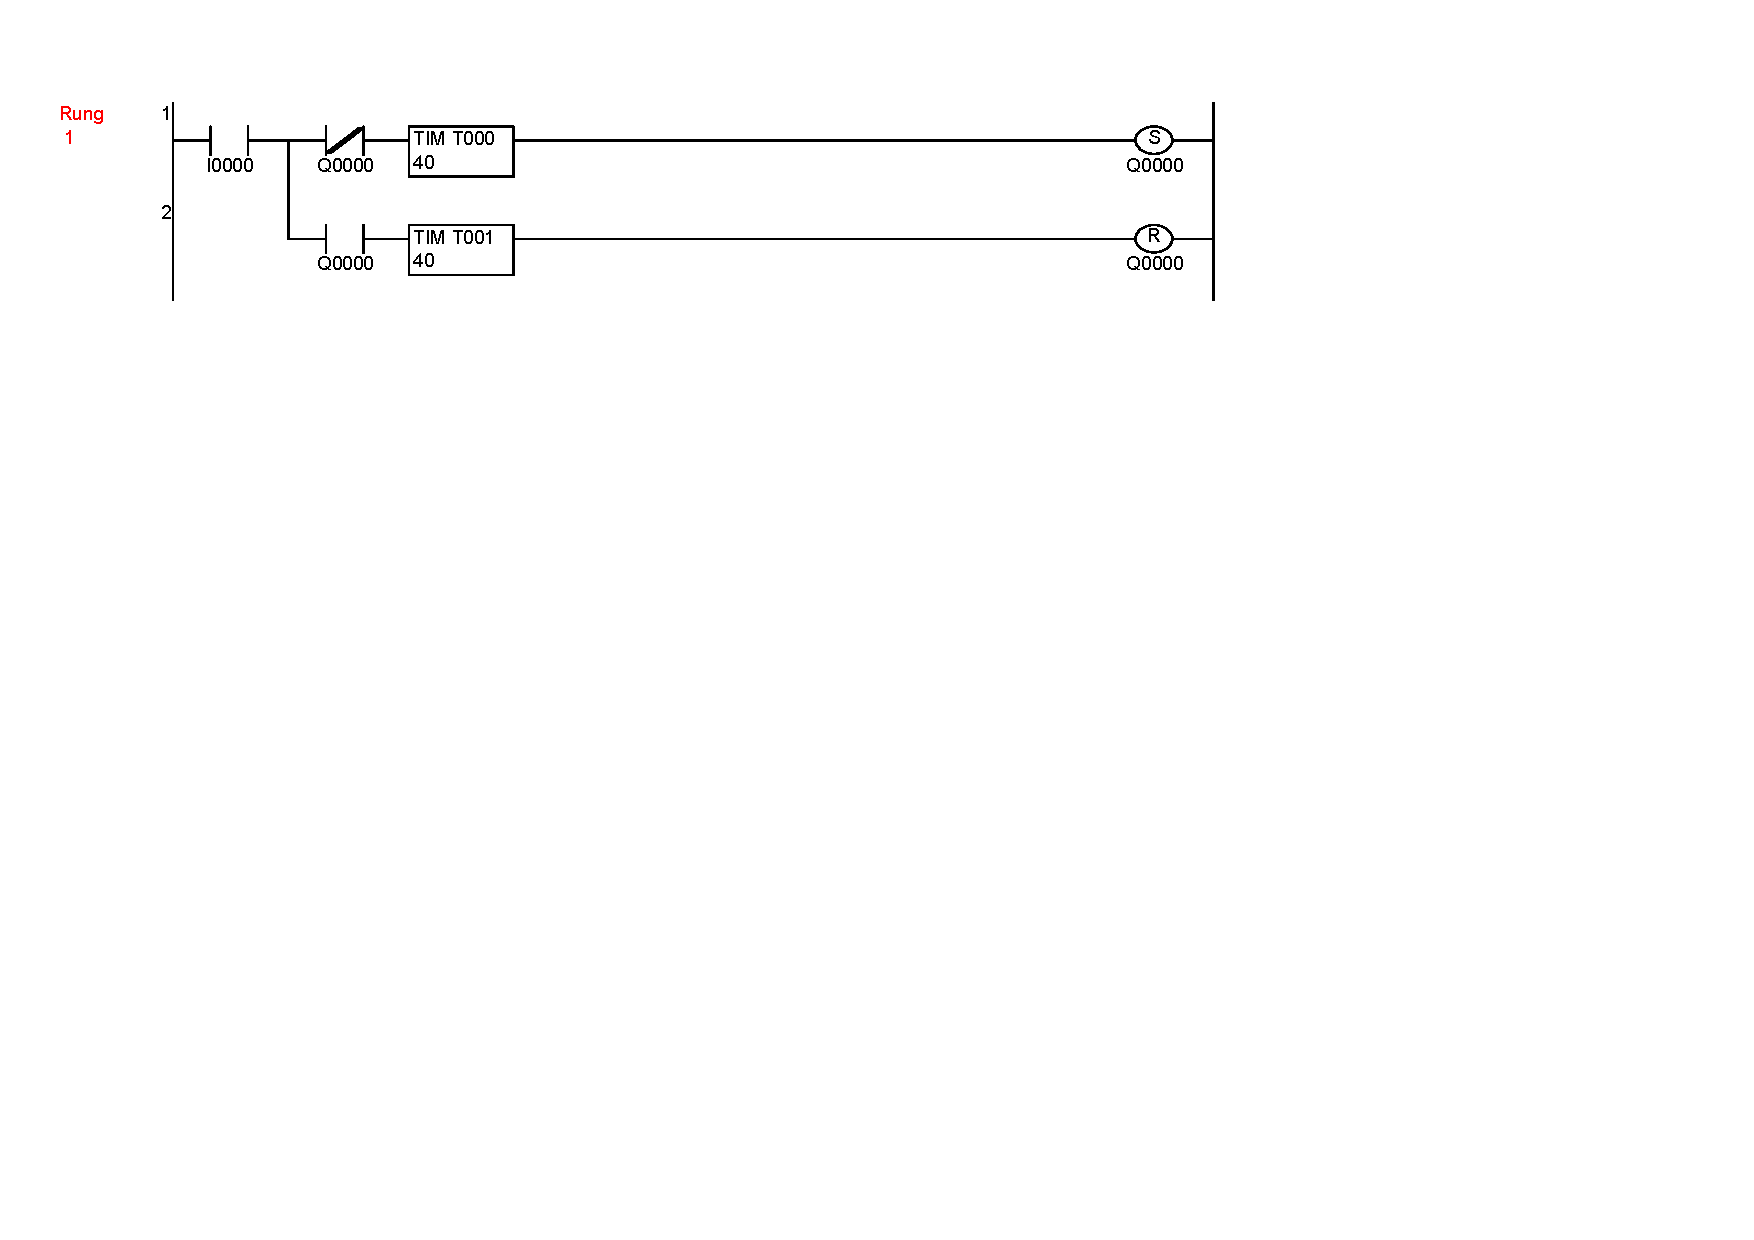
\includegraphics[trim={19pt 441pt 250pt 39pt}, clip, width=0.85\textwidth]{sources/diagramas/WINDLDR_tp3_ej13.pdf}
    \caption{Diagrama Ladder para oscilador cíclico de $4\,\text{s}$ (Ejercicio 13).}
    \label{fig.ej13:oscilador}
\end{figure}

\section{Ejercicio 14: Semáforo Secuencial Simple}
\textbf{Consigna:} Construya un semáforo que repita de forma cíclica la secuencia de luces con tiempos de $20\,\text{s}$,
$5\,\text{s}$ y $20\,\text{s}$.

\textbf{Análisis y Solución:}
Se implementa una cadena de tres temporizadores en cascada que activan en forma mutuamente excluyente las salidas
correspondientes a Verde, Amarillo y Rojo, reiniciando la secuencia automáticamente. El circuito Ladder completo se
representa en la figura \ref{fig.ej14:semaforo}.

\begin{figure}[!ht]
    \centering
    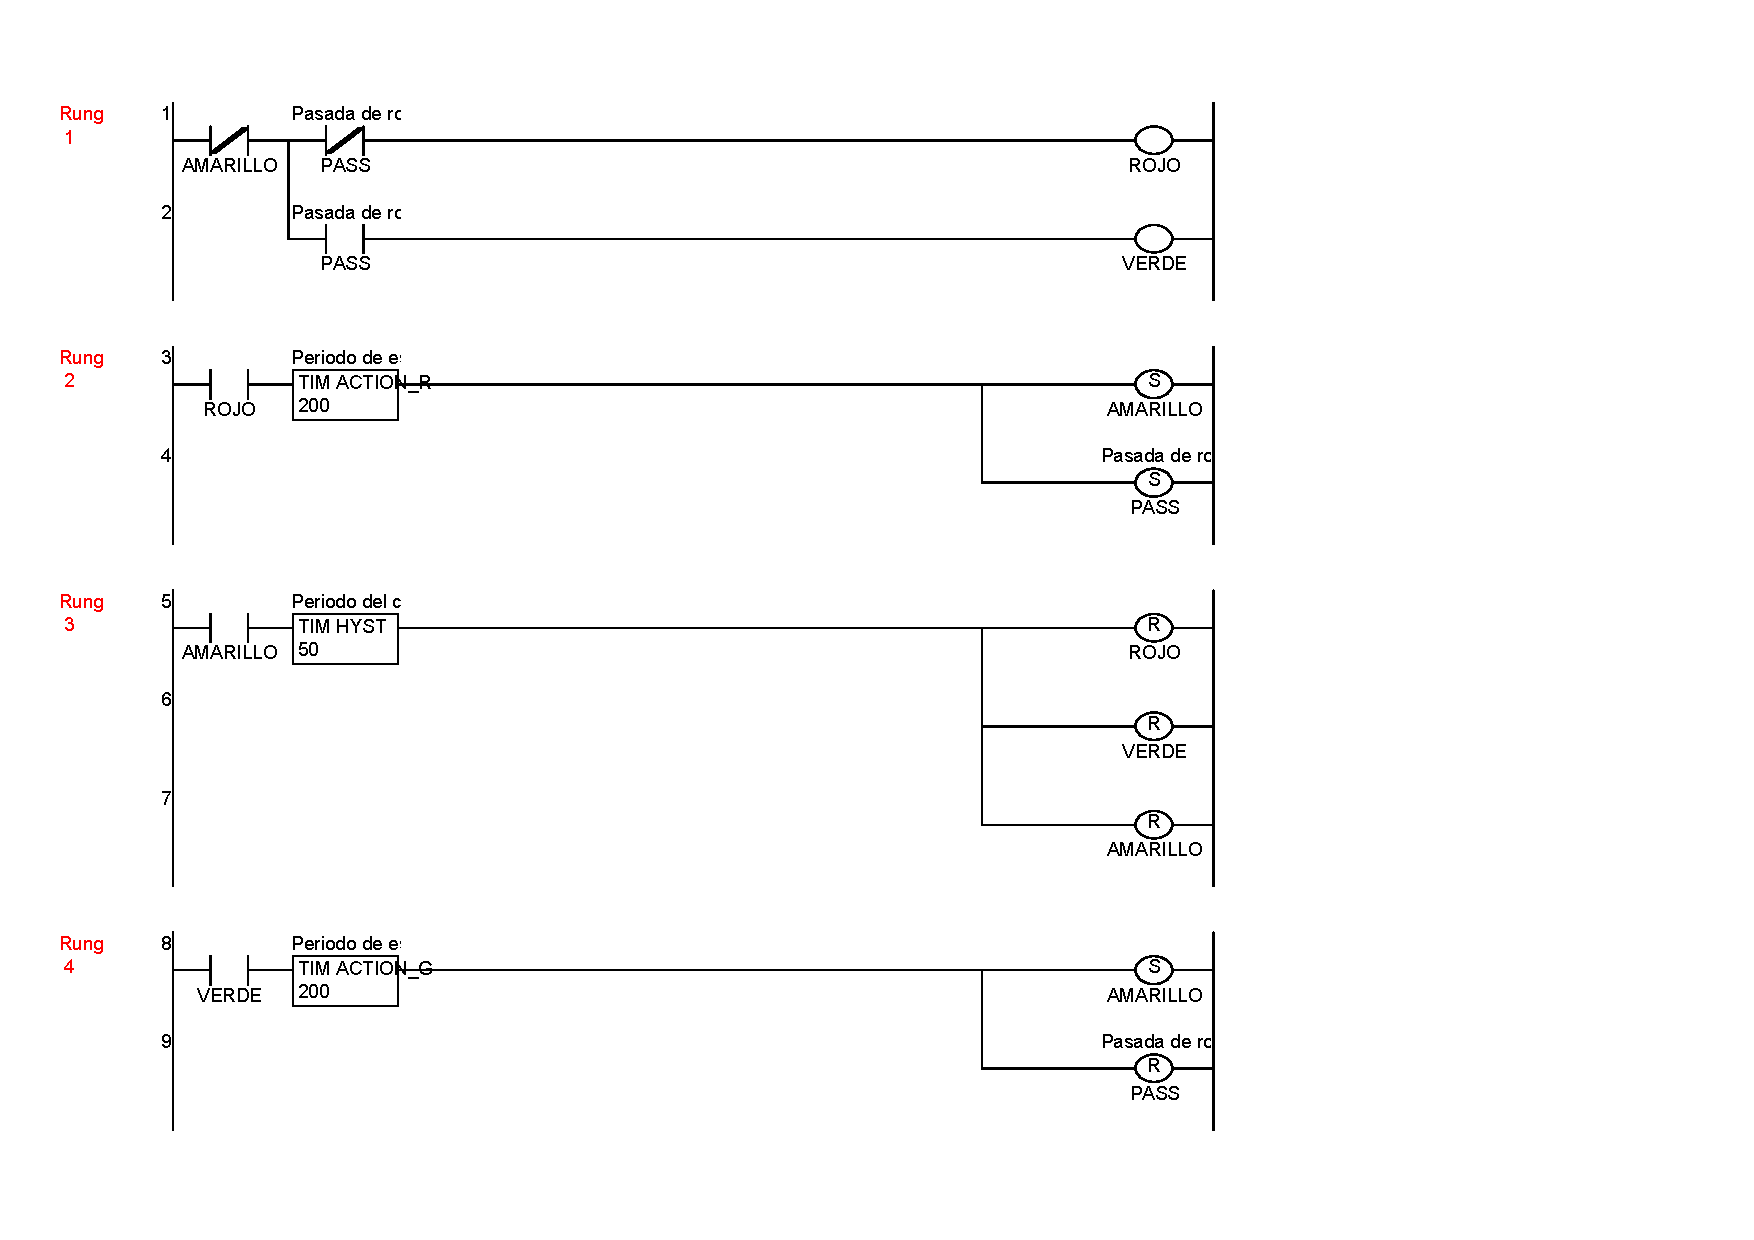
\includegraphics[trim={19pt 43pt 250pt 39pt}, clip, width=0.85\textwidth]{sources/diagramas/WINDLDR_tp3_ej14.pdf}
    \caption{Diagrama Ladder para Semáforo Secuencial (Ejercicio 14).}
    \label{fig.ej14:semaforo}
\end{figure}

\section{Ejercicio 15: Accionamiento de Grúa Industrial}
\textbf{Consigna:} Controlar el ciclo de trabajo de una grúa con electroimán entre dos posiciones de reposo mediante los
pulsadores A y B.

\textbf{Análisis y Solución:}
Se estructura un automatismo basado en secuencia de estados/marcas donde el ciclo 1 energiza el electroimán y traslada la
carga hasta la posición 2; posteriormente, el ciclo 2 retorna la grúa desenergizando el electroimán. La solución lógica se
presenta en la figura \ref{fig.ej15:grua}.

\begin{figure}[!ht]
    \centering
    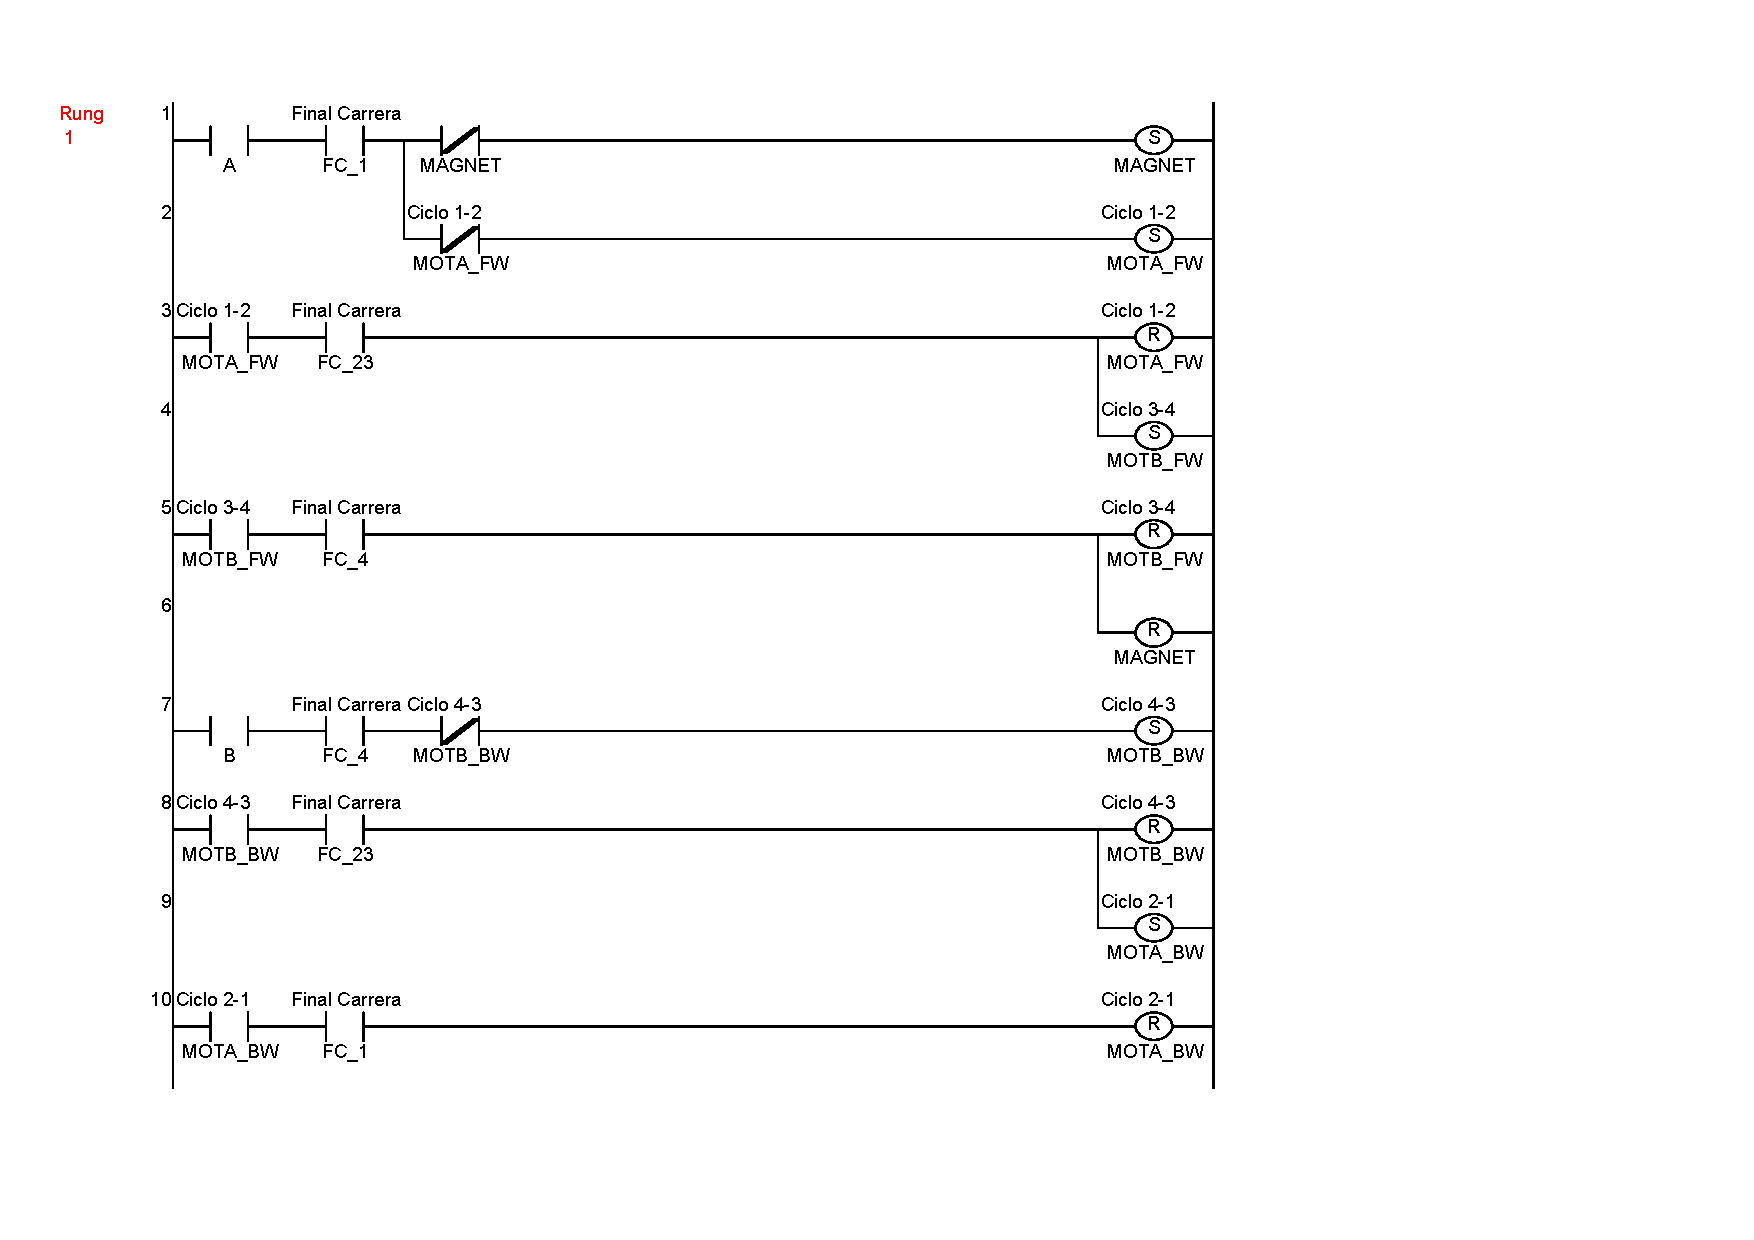
\includegraphics[trim={19pt 63pt 250pt 39pt}, clip, width=0.85\textwidth]{sources/diagramas/WINDLDR_tp3_ej15.pdf}
    \caption{Diagrama Ladder para el control de Grúa Industrial (Ejercicio 15).}
    \label{fig.ej15:grua}
\end{figure}

\section{Ejercicio 16: Ascensor de Tres Pisos}
\textbf{Consigna:} Controlar un ascensor de 3 pisos con sensores $Sa, Sb, Sc$ y botones $Pa, Pb, Pc$, activando las salidas
$Q0$ (subir) y $Q1$ (bajar).

\textbf{Análisis y Solución:}
Se compara la posición actual determinada por los finales de carrera con el piso solicitado, activando la salida de subida
o bajada con sus correspondientes enclavamientos hasta igualar la posición. El esquema Ladder se encuentra en la figura
\ref{fig.ej16:ascensor}.

\begin{figure}[!ht]
    \centering
    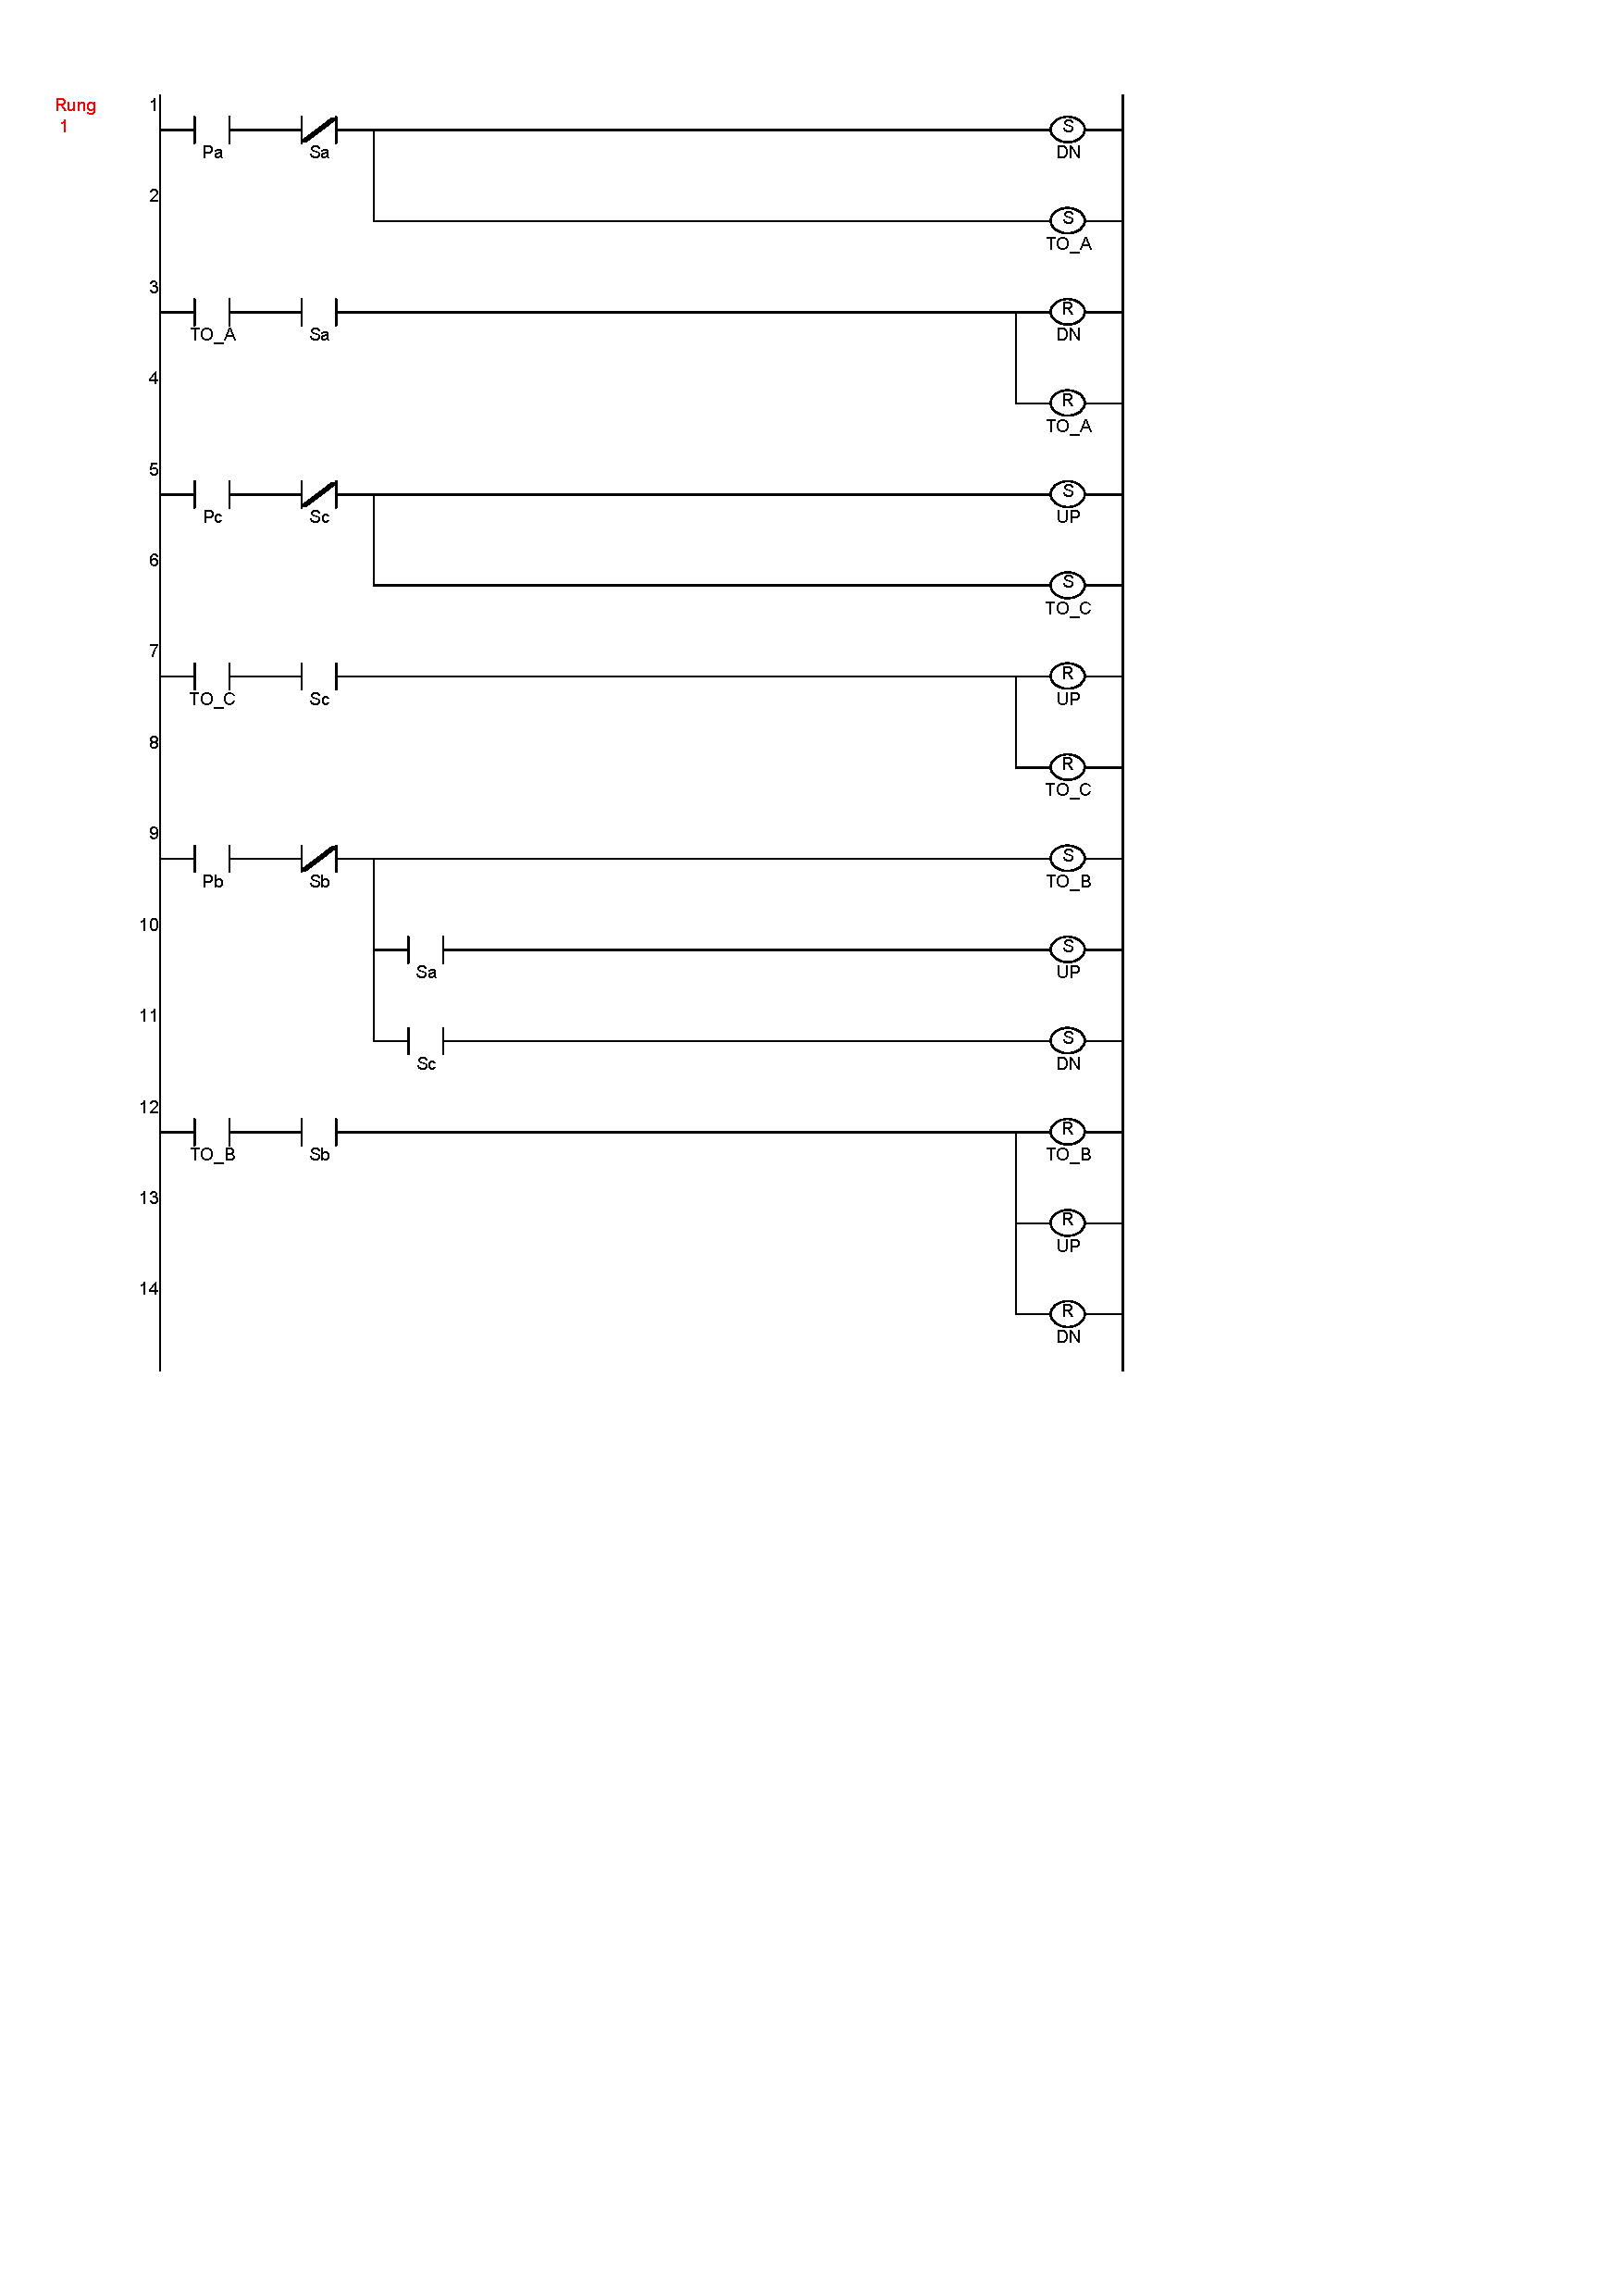
\includegraphics[trim={19pt 470pt 250pt 39pt}, clip, width=0.85\textwidth]{sources/diagramas/WINDLDR_tp3_ej16.pdf}
    \caption{Diagrama Ladder para Ascensor de Tres Pisos (Ejercicio 16).}
    \label{fig.ej16:ascensor}
\end{figure}

\section{Ejercicio 17: Semáforos Interconectados de Cruce de Calles}
\textbf{Consigna:} Controlar los semáforos de una intersección ($S1$ y $S2$) siguiendo la secuencia temporal requerida.

\textbf{Análisis y Solución:}
Se sincronizan las etapas de Verde, Amarillo y Rojo para ambas avenidas asegurando que no existan
luz verde en ambos sentidos simultáneamente, incluyendo los tiempos de seguridad. El diagrama se detalla en la
figura \ref{fig.ej17:cruce}.

\begin{figure}[!ht]
    \centering
    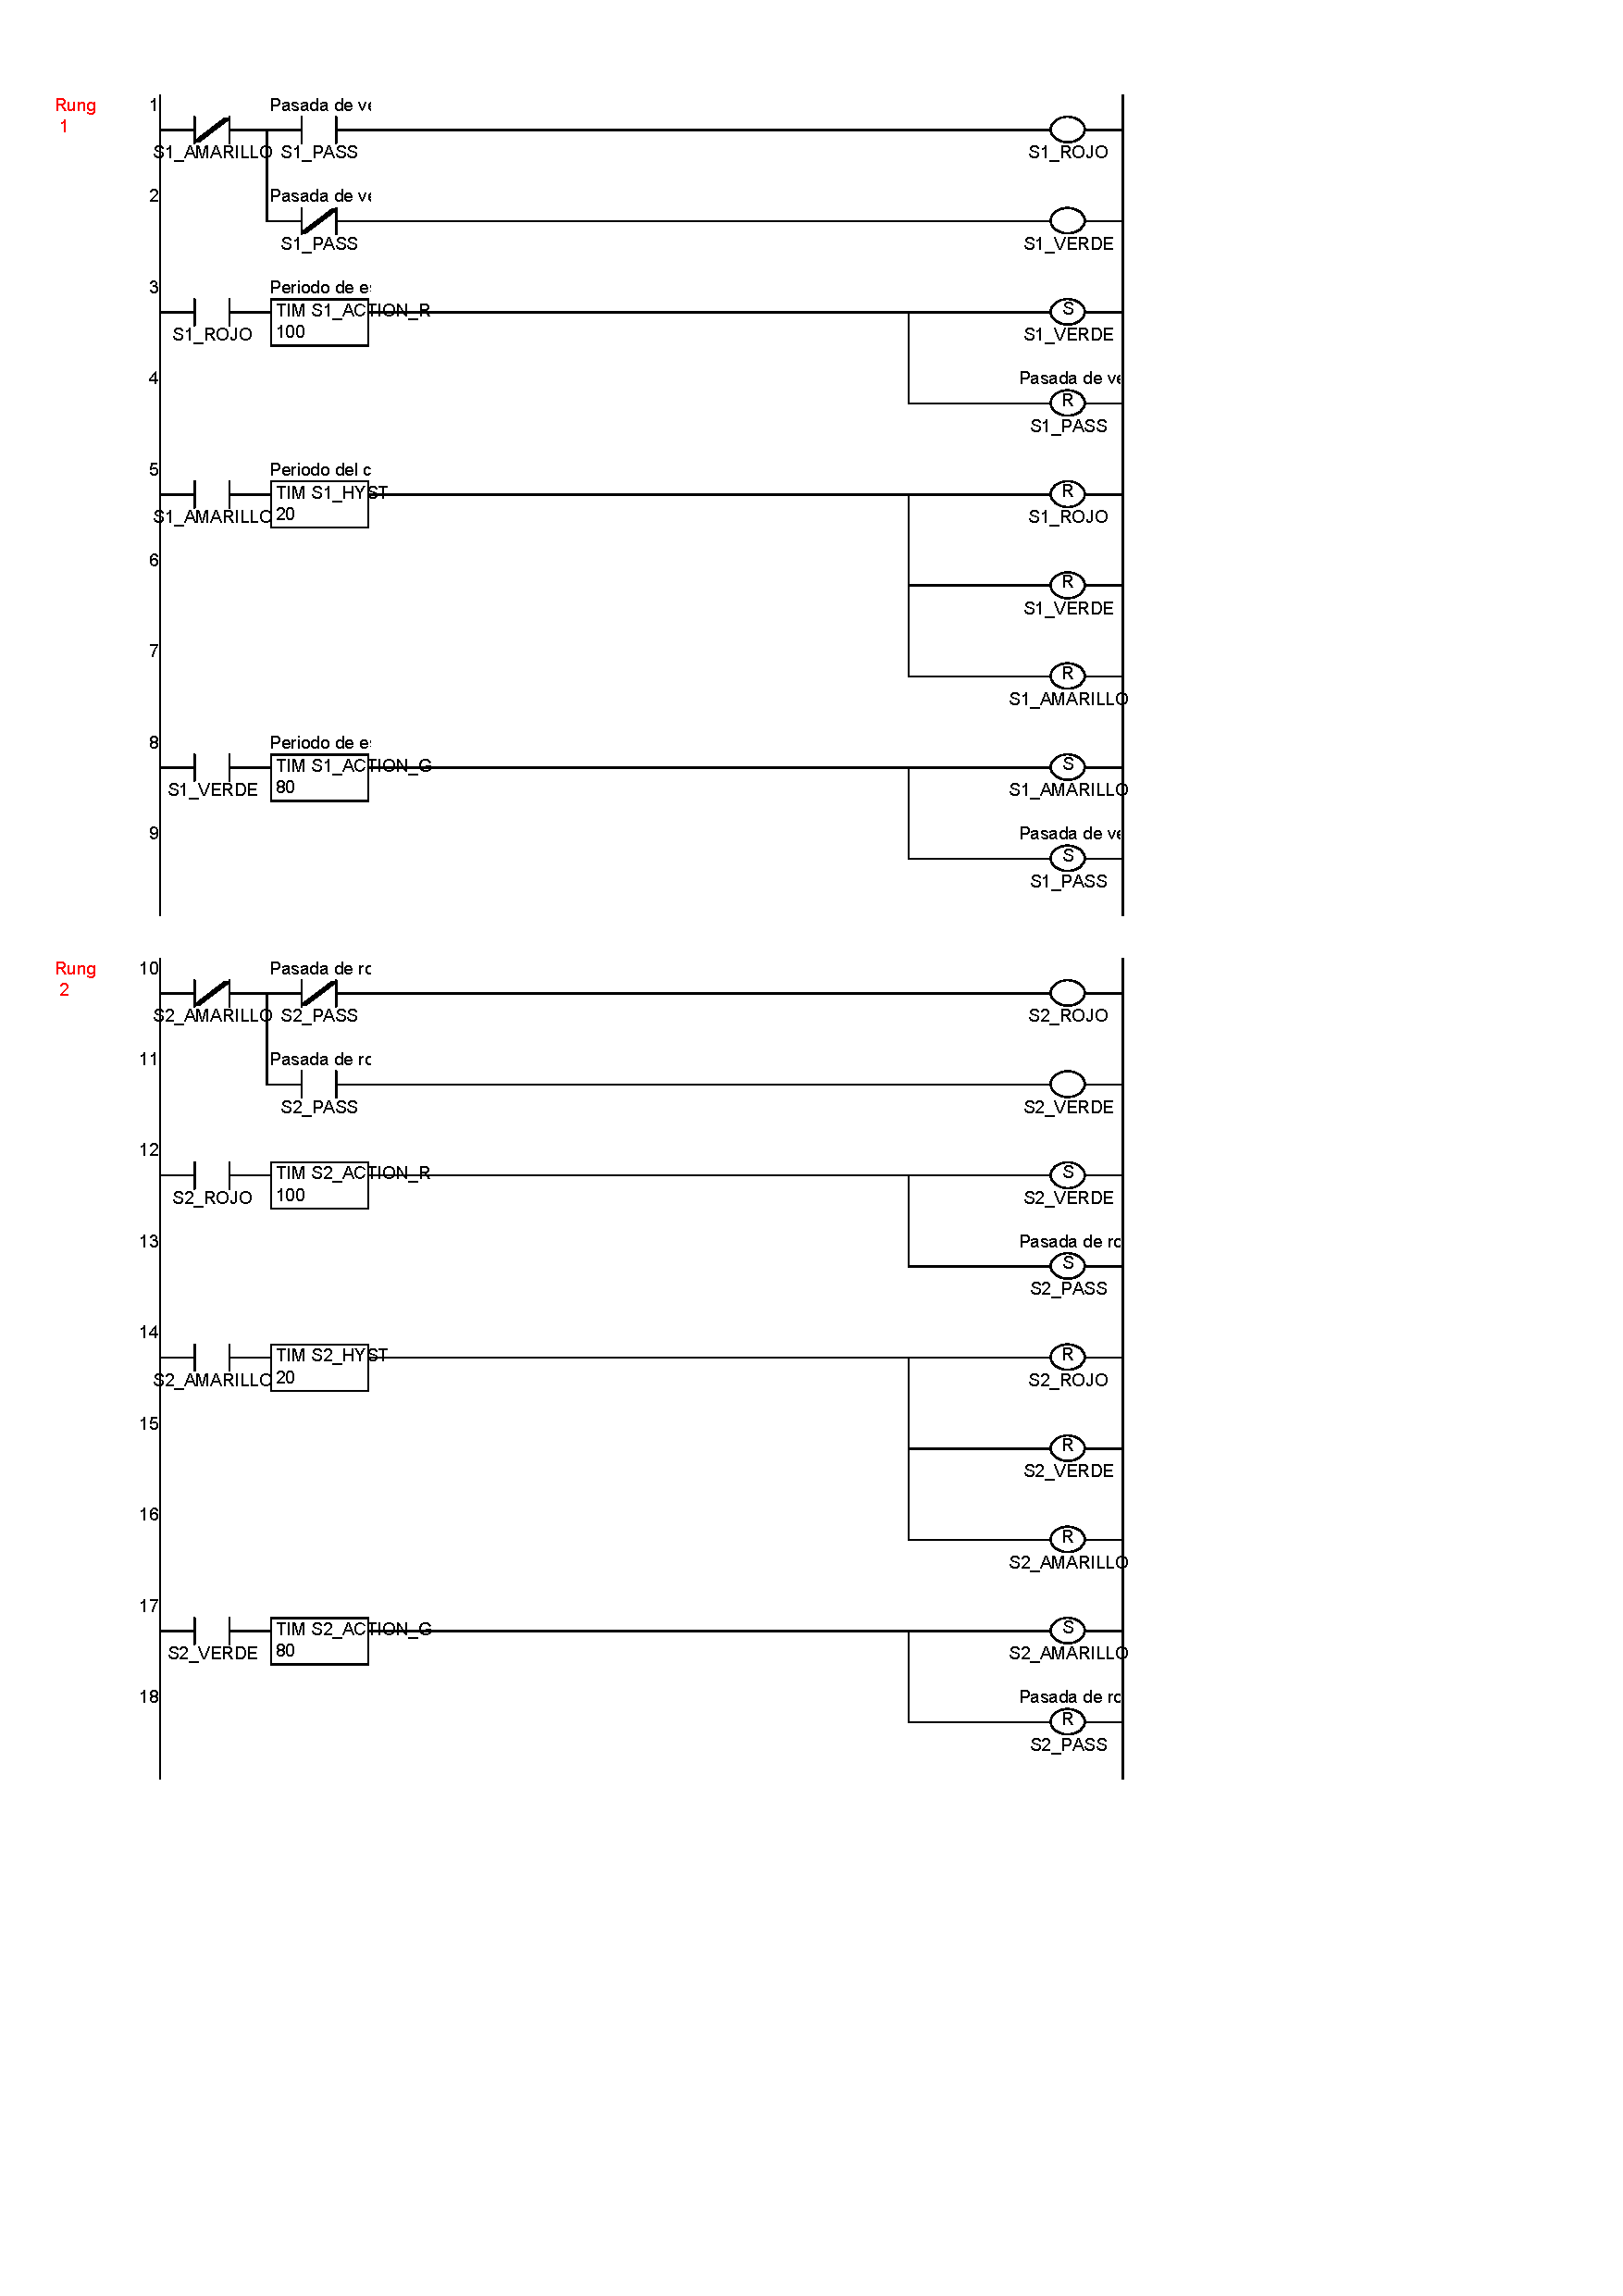
\includegraphics[trim={19pt 259pt 248pt 39pt}, clip, width=0.85\textwidth]{sources/diagramas/WINDLDR_tp3_ej17.pdf}
    \caption{Diagrama Ladder para Semáforos de Cruce de Calle (Ejercicio 17).}
    \label{fig.ej17:cruce}
\end{figure}
